\documentclass[12pt]{extarticle}
\usepackage{geometry}
\geometry{
a4paper,
total={170mm,257mm},
left=20mm,
top=20mm,
headheight=12pt
}
\usepackage[parfill]{parskip} % Activate to begin paragraphs with an empty line rather than an indent
\usepackage{graphicx} % Use pdf, png, jpg, or eps§ with pdflatex; use eps in DVI mode
% TeX will automatically convert eps --> pdf in pdflatex
		
\usepackage{amssymb,amsmath,amsthm}
\usepackage{commath}
\usepackage{longtable}
\usepackage[hyphens]{url}
\usepackage[dvipsnames]{xcolor}
\usepackage[unicode=true,colorlinks=true,urlcolor=CadetBlue,citecolor=black,linkcolor=black]{hyperref}
\usepackage{booktabs}
\usepackage{pgfplotstable} 
\PassOptionsToPackage{hyphens}{url} % url is loaded by hyperref
\usepackage{authblk}
\usepackage{subcaption}
\captionsetup[subfigure]{labelformat=empty}
\usepackage[font=small,labelfont=bf]{caption}
\usepackage{longtable}
\usepackage{gensymb,siunitx}
\usepackage{cleveref}

%SetFonts
% newtxtext+newtxmath
\usepackage{newtxtext} %loads helv for ss, txtt for tt
\usepackage{amsmath}
\usepackage[bigdelims]{newtxmath}
\usepackage[T1]{fontenc}
\usepackage{textcomp}
%SetFonts

\renewcommand{\baselinestretch}{1.5}

% less space before sections 
% \@startsection {NAME}{LEVEL}{INDENT}{BEFORESKIP}{AFTERSKIP}{STYLE} 
%            optional * [ALTHEADING]{HEADING} 
\makeatletter
 \renewcommand\section{\@startsection {section}{1}{\z@}%
     {-2.5ex \@plus -1ex \@minus -.2ex}%
     {1.3ex \@plus.2ex}%
    {\Large\bfseries}}
    
% Species names
%% Meta-Command for defining new species macros
\usepackage{xspace}

\newcommand{\species}[3]{%
  \newcommand{#1}{\gdef#1{\textit{#3}\xspace}\textit{#2}\xspace}}
  
\species{\yeast}{Saccharomyces cerevisiae}{S.~cerevisiae}
\species{\calbicans}{Candida albicans}{C.~albicans}
\species{\cneoformans}{Cryptococcus neoformans}{C.~neoformans}

% Yoav & Lee commands
\newcommand*{\tr}{^\intercal}
\let\vec\mathbf
\newcommand{\matrx}[1]{{\left[ \stackrel{}{#1}\right]}}
\newcommand{\diag}[1]{\mbox{diag}\matrx{#1}}
\newcommand{\goesto}{\rightarrow}
\newcommand{\dspfrac}[2]{\frac{\displaystyle #1}{\displaystyle #2} }
\newtheorem{theorem}{Theorem}
\newtheorem{corollary}{Corollary}
\newtheorem{lemma}{Lemma}
\newtheorem{remark}{Remark}
\newtheorem{result}{Result}
\renewcommand\qedsymbol{} % no square at end of proof
\newcommand{\cl}{\mathbf{L}}
\newcommand{\cj}{\mathbf{J}}
\newcommand{\ci}{I}
\newcommand{\likelihood}{\mathcal{L}}

% genotype commands
\newcommand{\euwt}{\emph{2n}}
\newcommand{\anwt}{\emph{2n+1}}
\newcommand{\eumt}{\emph{2n*}}
\newcommand{\anmt}{\emph{2n+1*}}

% Supplementary
\newcommand{\beginsupplement}{%
      	\setcounter{table}{0}
        \renewcommand{\thetable}{S\arabic{table}}%
        \setcounter{figure}{0}
        \renewcommand{\thefigure}{S\arabic{figure}}%
}

% NatBib
\usepackage[round,colon,authoryear]{natbib}

% Title page
% Chromosomal duplication is a transient evolutionary solution to stress
%\title{Clonal interference between aneuploidy and mutation}
\title{Adaptive evolution with aneuploidy and mutation}

% Authors
\renewcommand\Affilfont{\small}

\author[1,*]{Ilia Kohanovski}
\author[2,*]{Martin Pontz}
\author[3]{Avihu H. Yona}
%\author[d]{Orna Dahan}
%\author[d]{Yitzhak Pilpel}
\author[1,2,$\dagger$]{Yoav Ram}

\affil[1]{School of Computer Science, Reichman University, Herzliya, Israel}
\affil[2]{School of Zoology, Faculty of Life Sciences, Tel Aviv University, Tel Aviv, Israel}
\affil[3]{Institute of Biochemistry, Food Science and Nutrition,
Robert H. Smith Faculty of Agriculture, Food and Environment,
The Hebrew University of Jerusalem, Israel}
%\affil[d]{Department of Molecular Genetics, Weizmann Institute of Science, Rehovot 76100, Israel}
\affil[*]{These authors contributed equally to this work}
\affil[$\dagger$]{Corresponding author: yoav@yoavram.com}

% Document
\begin{document}
\maketitle

% Abstract
\begin{abstract}
Aneuploidy is common in eukaryotes, often leading to decreased cell growth and fitness. However, evidence from yeast and fungi, as well as human tumour cells, suggests that aneuploidy can be beneficial under stressful conditions and lead to elevated growth rates and adaptation.
Importantly, aneuploidy differs from point mutations in rate, fitness effect, and reversibility.
Here, we develop evolutionary models for adaptive evolution with both mutation and aneuploidy. 
These models are used within an approximate Bayesian computation framework to estimate the formation rate and fitness effect of aneuploidy and mutation from  results of evolutionary experiments in which \yeast adapted to heat stress: the experimental populations first acquired chromosome duplications, only to later revert back to a euploid state.
We also analyze our models to estimate the effect of the aneuploidy and mutation rates on the expected adaptation time and the probability for adaptation via aneuploidy.
Our results suggest that aneuploidy can be a transient adaptive solution, which can decelerate adaptation in a non-intuitive manner. By creating an evolutionary conflict between the individual and the population, aneuploidy further complicates the process of adaptation in cell populations.
\end{abstract}

% TODO cite https://www.biorxiv.org/content/10.1101/2020.10.07.327759v1
% cite: https://www.cell.com/developmental-cell/fulltext/S1534-5807(21)00562-1?_returnURL=https%3A%2F%2Flinkinghub.elsevier.com%2Fretrieve%2Fpii%2FS1534580721005621%3Fshowall%3Dtrue
% cite: https://www.cell.com/developmental-cell/fulltext/S1534-5807(21)00592-X?_returnURL=https%3A%2F%2Flinkinghub.elsevier.com%2Fretrieve%2Fpii%2FS153458072100592X%3Fshowall%3Dtrue

\pagebreak
% Introduction
\section*{Introduction}

\paragraph*{Aneuploidy is common in eukaryotes.}
Aneuploidy is an imbalance in the number of chromosomes in the cell: an incorrect karyotype.
Evidence suggests aneuploidy is very common in eukaryotes, e.g. animals~\citep{Santaguida2015review, Naylor2016, Bakhoum2017}, and fungi~\citep{Pavelka2010, Zhu2016, Robbins2017, Todd2017}.
Aneuploidy has been implicated in cancer formation and progression~\citep{Boveri2008, Schvartzman2010}: 
90\% of solid tumours and 50\% of blood cancers are aneuploid~\citep{Santaguida2015review}.
Aneuploidy is also linked to the emergence of drug resistance~\citep{Selmecki2009} and virulence~\citep{Moller2018} in fungal pathogens, which are under-studied~\citep{Rodrigues2018} despite infecting close to a billion people per year, causing serious infections and significant morbidity in >150 million people per year and killing >1.5 million people per year~\citep{Selmecki2009, Rodrigues2018}.
In addition, aneuploidy is common in protozoan pathogens of the Leishmania genus, a major global health concern~\citep{Mannaert2012}.

\paragraph*{Aneuploidy is generally deleterious.}
The molecular and genetic mechanisms involved in aneuploidy have been explored~\citep{Musacchio2007, Sheltzer2011, Chen2012b, Rancati2013, Gerstein2015, Shor2015}.
Experiments with human and mouse embryos found that aneuploidy is usually lethal.
It is also associated with developmental defects and lethality in other multicellular organisms~\citep{Sheltzer2011}. For example, aneuploid mouse embryonic cells grow slower than euploid cells~\citep{Williams2008}.
Similarly, in unicellular eukaryotes growing in benign conditions, aneuploidy usually leads to slower growth and decreased overall fitness~\citep{Niwa2006, Torres2007, Pavelka2010, Sheltzer2011, Kasuga2016}, in part due to proteotoxic stress caused by increased expression in aneuploid cells~\citep{Pavelka2010, Santaguida2015, Zhu2018} and hypo-osmotic-like stress~\citep{Tsai2019}.
% TODO cite Yang, F. et al. The fitness costs and benefits of trisomy of each Candida albicans chromosome. Genetics 218, 1–7 (2021).

\paragraph*{Aneuploidy can lead to adaptation.}
However, aneuploidy can be beneficial under stressful conditions due to the wide range of phenotypes it can produce, some of which are advantageous~\citep{Pavelka2010}.
Thus, aneuploidy can lead to rapid adaptation in unicellular eukaryotes~\citep{Gerstein2015,Torres2010, Hong2014, Rancati2008}, as well as to rapid growth of somatic tumour cells~\citep{Schvartzman2010, Sheltzer2017}.
For example, aneuploidy in \yeast facilitates adaptation to a variety of stressful conditions like heat and pH~\citep{Yona2012}, copper~\citep{Covo2014, Gerstein2015}, salt~\citep{Dhar2011}, and nutrient limitation~\citep{Dunham2002, Gresham2008}.
Importantly, aneuploidy can also lead to drug resistance in pathogenic fungi such as \calbicans~\citep{Selmecki2008, Selmecki2010, Gerstein2018} and \cneoformans~\citep{Sionov2010}, which cause candidiasis and meningoencephalitis, respectively.

\paragraph*{Transient adaptive solution.} 
Aneuploidy differs from mutation due to its distinct properties. 
Chromosome duplication usually occurs more often than mutation and on average produces larger fitness effects.
Yet, because it affects many genes on a whole chromosome or a chromosome fragment, aneuploidy also carries fitness costs.
Thus, aneuploidy can be a \emph{transient adaptive solution}: it can rapidly occur and fix in the population under stressful conditions, and can be rapidly lost when the cost outweighs the benefit---when stress is removed or after beneficial mutations occur.
Experimental evidence of such a transient role of aneuploidy was demonstrated by \citet{Yona2012}. They evolved populations of \yeast under strong heat or pH stress.
The populations adapted to the heat and pH stress within 450 and 150 generations, and this adaptation was determined to be due to chromosome duplications.
Much later, after more than 1500 and 750 generations, for the heat and pH stress, respectively, the populations reverted back to an euploid state, while remaining adapted to the stress and accumulating multiple mutations.
However, under gradual heat stress, aneuploidy was not observed.
\citet{Yona2012} concluded that aneuploidy serves as a transient adaptive solution, or a ``quick fix'', which is expected to facilitate adaptation. 

\paragraph*{The present study.}
Here, we develop an evolutionary-genetic model that includes the effects of natural selection, genetic drift, aneuploidy, and mutation to examine the role of aneuploidy in adaptive evolution.
This model follows a population of cells characterised by both their ploidy and their genotype.
We fit this model to the experimental results of \citet{Yona2012} using an \emph{approximate Bayesian computation} framework~\citep{Sisson2009} to infer model parameters, including selection coefficients and rates of aneuploidy and mutation, and to test hypotheses about the evolutionary process by performing model selection between different versions of the model.
%We also mathematically analyze this evolutionary-genetic model to estimate the effects of selection, mutation, and aneuploidy on the adaptation time and the probability for adaptation via aneuploidy.


%%%%%%%%%%%%%%%%%%%%%%%%
% Models and Methods
\section*{Models and Methods}

%%%%%%%% Fig illustation
\begin{figure}[b!]
  \centering
  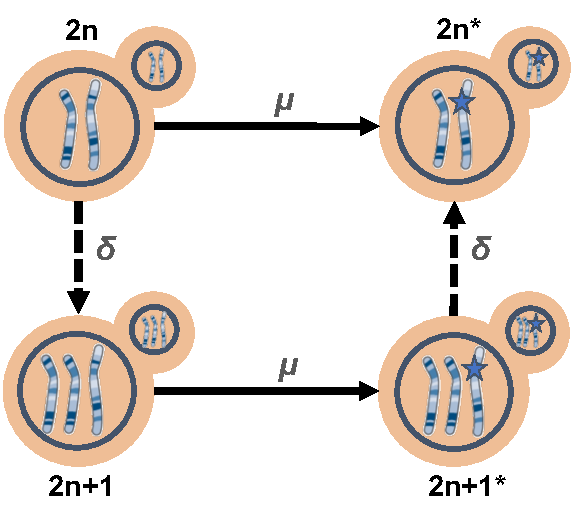
\includegraphics[height=1.8in]{../figures/Fig1-A.pdf}      
  \label{fig:model1}
  \caption{
    \textbf{Model illustration.}
    There are four genotypes in our model: euploid wild-type, \euwt; euploid mutant, \eumt; aneuploid wild-type, \anwt; and aneuploid mutant, \anmt.
    Overall there are two possible trajectories from \euwt\; to \eumt.
    Arrows denote transitions between genotypes, with transitions rates: $\mu$, beneficial mutation rate; $\delta$, aneuploidy rate.
  }
  \label{fig:models}
\end{figure}
%%%%%%%%%%%%%%%%%%%%%%%%

%%%%%%%%%%%%%%%%%%%%%%%%
\paragraph*{Evolutionary Model.}
We model the evolution of a population of cells using a Wright-Fisher model~\citep{Otto2007}, assuming a constant effective population size $N$, non-overlapping generations, and including the effects of natural selection, genetic drift, aneuploidy, and mutation. 
We focus on beneficial genetic modifications, neglecting the effects of deleterious and neutral mutations or karyotypic changes.
The model allows for a single aneuploid karyotype (e.g., chromosome III duplication) and a single mutation to accumulate in the genotype.
Thus, the model follows four genotypes~(\Cref{fig:models}): euploid wild-type, \euwt, the initial genotype; 
euploid mutant, \eumt, with the standard karyotype and a single beneficial mutation; 
aneuploid wild-type, \anwt, with an extra chromosome, i.e., following chromosome duplication; and
aneuploid mutant, \anmt, with and extra chromosome and a beneficial mutation. 

Transitions between the genotypes occur as follows~(\Cref{fig:models}A): Beneficial mutations from \euwt\; to \eumt\; and from \anwt\; to \anmt\; occur with probability $\mu$, the mutation rate. We neglect back-mutations (i.e., from \eumt\; to \euwt\; and from \anmt\; to \anwt).
Aneuploidy is formed by chromosome mis-segregation, so that cells transition from \euwt\; to \anwt\; and from \anmt\ to \eumt\ with probability $\delta$, the aneuploidy rate. That is, we assume chromosomes are gained and lost at the same rate, and we neglect events that form a less-fit genotype (i.e., \anwt\; to \euwt\; and \eumt\; to \anmt).
The fitness values of the four genotypes are given by \Cref{table:fitness}.

%%% Table: fitness
\begin{table}[h]
\centering
\caption{\textbf{Fitness values.}}
\begin{tabular}{lllll}
\emph{Genotype} $i$ & \euwt & \anwt & \anmt & \eumt \\
\hline
\emph{Fitness} $w_i$ & $1$ & $1-c+b$ & $(1-c)(1+s)+b$ & $1+s$               
\end{tabular}
\label{table:fitness}
\caption*{
$s \ge 0$ is the selection coefficient of a beneficial mutation;
$0 \le c \le 1$ is the fitness cost of aneuploidy;
and $b \ge c$ is the selection coefficient, or fitness benefit, of aneuploidy.
}
\end{table}
%%%%%%%%%%%%%%%%%%%%%%%%

The initial population has $N$ cells with genotype \euwt.
The effect of natural selection on the frequency $f_i$ of genotype $i = 2n, 2n+1, 2n+1^*, \text{or } 2n^*$ is given by
    \begin{equation} \label{eq:selection-single} 
      f^s_i = \frac{f_i w_i}{\bar{w}} \;,
    \end{equation}
where the fitness values $w_i$ are given in \Cref{table:fitness} and $\bar{w} = \sum_{j}{f_j w_j}$ is the population mean fitness.
The effect of mutation and aneuploidy on genotype frequencies is given by
    \begin{equation} \label{eq:mutation-aneuploidy-single}
    \begin{aligned}
      &f^m_{2n} &=&\; (1 - \delta - \mu) f^s_{2n}  \;,\\
      &f^m_{2n+1} &=&\; \delta f^s_{2n} + (1 - \mu) f^s_{2n+1}  \;,\\
      &f^m_{2n+1^*} &=&\; \mu f^s_{2n+1} + (1-\delta) f^s_{2n+1^*}  \;,\\
      &f^m_{2n^*} &=&\; \mu f^s_{2n} + \delta f^s_{2n+1} + f^s_{2n^*}  \;.
    \end{aligned}
    \end{equation}
Finally, random genetic drift is modeled using a multinomial distribution~\citep{Otto2007},
    \begin{equation} \label{eq:drift-single}
      \vec{f'} \sim \frac{1}{N} \cdot \mathit{Mult}(N,\ \vec{f^m}) \;,
    \end{equation}
where $\vec{f^m}=(f^m_{2n}\ ,\ f^m_{2n+1}\ ,\ f^m_{2n+1^*}\ ,\ f^m_{2n^*})$ are the frequencies of the genotypes after mutation and aneuploidy, $\vec{f'}$ are the genotype frequencies in the next generation, and $Mult(N,\ \vec{f})$ is a multinomial distribution parameterized by the population size $N$ and the genotype frequencies $\vec{f}$.
Overall, the change in genotype frequencies from one generation to the next is given by the transformation $f_i \to f'_i$.


\paragraph{Empirical evidence.}

We use the results of evolutionary experiments reported by \citet{Yona2012}.
In their heat-stress experiment, four populations of \yeast evolved under \SI{39}{\celsius}. Aneuploidy fixed in all four population in the first 450 generations (hereafter, fixation or elimination of a genotype \emph{by generation $t$} means that more than 95\% or less than 5\% of the population carry the genotype at generation $t$, and possibly earlier). 
From re-analysis of data not published in the original paper, aneuploidy did not fix before at least 200 generations elapsed.
The experiment continued with two populations, in which aneuploidy was eliminated by generation 1,700 and 2,350 while still under the same conditions of elevated heat (\SI{39}{\celsius}).


\paragraph{Likelihood function.} 
Because our model, just like the Wright-Fisher model, is non-linear and stochastic, computing the distribution of fixation time $T(g)$ of genotype $g$ for use in the likelihood function is intractable (it is even hard to use a diffusion-equation approximation due to the model having multiple genotypes, rather than just two).
We overcome this problem by approximating the likelihood using simulations. We simulate 1,000 experiments per parameter vector $\theta = (\mu, \delta, s, b, c)$, resulting in a set of simulated observations $\tilde{\vec X} = \{\tilde{X}_i\}_{i=1}^{1000}$. We then compute the approximate likelihood,
\begin{equation}\begin{aligned}
\label{eq:heatstress-likelihood}
\likelihood(\theta) = &\ P^4(200 \le T(2n+1) \le 450) \cdot 
	\Big[1 - \\
	&	P_{\tilde{\vec X}}^4\big(!\{T(2n^*)<1700\} \mid 200 \le T(2n+1) \le 450\big)- \\
	&	P_{\tilde{\vec X}}^4\big(!\{1700 < T(2n^*) < 2350\} \mid 200 \le T(2n+1) \le 450\big)+ \\
	&	P_{\tilde{\vec X}}^4\big(!\{T(2n^*)<1700\} \land !\{1700 < T(2n^*) < 2350\} \mid 200 \le T(2n+1) \le 450\big) 
	\Big]\;,
\end{aligned}\end{equation}
where $!\{\ldots\}$ is the "logical not" operator, $P^4(\ldots)$ is the 4th power of $P(\ldots)$, and all probabilities $P_{\tilde{\vec X}}(\ldots)$ are approximated from the results of the simulations $\tilde{\vec X}$. For example, $P_{\tilde{\vec X}}\big(!\{T(2n^*)<1700\} \mid 200 \le T(2n+1) \le 450\big)$ is approximated by taking simulations in which \anwt\; fixed before generation 450 but not before generation 200, and computing the fraction of such simulations in which \eumt\; did not fix by generation 1,700, and hence aneuploidy did not extinct before generation 1,700.
\Cref{fig:seeds} compares results with less and more simulated experiments, demonstrating that 1,000 simulations are likely sufficient.
 
For a model without aneuploidy (that is, when the aneuploidy rate is fixed at zero, $\delta=0$), we disregard the increased expression in chromosome III and the growth advantage measured in generation 450, and focus on the growth advantage measured in later generations, presumably due to a beneficial mutation. 
Therefore, the likelihood is approximated by
\begin{equation}\begin{aligned}
\label{eq:heatstress-noaneuploidy-likelihood}
\likelihood_{!}(\theta) = &\ 
	1 - 
	P_{\tilde{\vec X}}^4\big(!\{T(2n^*)<1700\}\big) - \\
&	P_{\tilde{\vec X}}^4\big(!\{1700 < T(2n^*) < 2350\}\big) + \\
&	P_{\tilde{\vec X}}^4\big(!\{T(2n^*)<1700\} \land !\{1700 < T(2n^*) < 2350\}\big)
\;.
\end{aligned}\end{equation}

\paragraph{Parameter inference.} To infer model parameters, we use approximate Bayesian computation with a sequential Monte-Carlo scheme, or ABC-SMC~\citep{Sisson2009}, implemented in the \texttt{pyABC} Python package~\citep[\href{https://pyabc.readthedocs.io}{pyabc.readthedocs.io}]{Klinger2018}.
This approach uses numerical stochastic simulations of the model to infer a posterior distribution over the model parameters. It is a method of likelihood-free, simulation-based inference~\citep{Cranmer2020}, that is, for estimating a posterior distribution when a likelihood function cannot be directly computed. It is therefore suitable in our case, in which the likelihood function can only be approximated from simulations, and cannot be directly computed. 

The ABC-SMC algorithm employs sequential importance sampling over multiple iterations~\citep{Toni2009, Klinger2017, Syga2021}.
In iteration $t$ of the algorithm, a set of parameter vectors, $\{\theta_{i,t}\}_{i=1}^{n_t}$, also called \emph{particles}, are constructed in the following way.
A proposal particle, $\theta^*$, is sampled from a proposal distribution, and is either accepted or rejected, until $n_t$ particles are accepted.
The number of particles, $n_t$, is adapted at every iteration $t$ using the adaptive population strategy~\citep[\href{https://pyabc.readthedocs.io}{pyabc.readthedocs.io}]{Klinger2018}.
For $t=0$, the proposal particle is sampled from the prior distribution, $p(\theta)$.
For $t>0$, the proposal particle is sampled from the particles accepted in the previous iteration, $\{\theta_{i,t-1}\}_{i=1}^{n_{t-1}}$, each with a probability relative to its weight $W_{t-1}(\theta_{i,t-1})$ (see below). The proposal particle is then perturbed using a kernel perturbation kernel, $K_t(\theta^* \mid \theta)$ where $\theta$ is the sample from the previous iteration.
Then, a set of synthetic observations $\tilde{\vec X}^*$ is simulated, and the proposal particle $\theta^*$ is accepted if its approximate likelihood (\cref{eq:heatstress-likelihood}) is high enough, $\likelihood(\theta^*)>1-\epsilon_t$ (or more commonly, if $1-\likelihood(\theta^*) < \epsilon_t$), where $\epsilon_t>0$ is the \emph{acceptance threshold}, as higher values of $\epsilon_t$ allow more particles to be accepted. 
The acceptance threshold $\epsilon_t$ is chosen as the median of the $1-\likelihood(\theta)$ of the particles accepted in the previous iteration, $t-1$, and $\epsilon_0=0.01$. 
For each accepted particle $\theta_{i,t}$ a weight $W_t(\theta_{i,t})$ is assigned: for $t=0$, $W_0(\theta_{i,0})=1$, and for $t>0$, 
$W_t(\theta_{i,t}) = p(\theta_{i,t}) / \sum_{i=1}^{n_{t-1}}{W_{t-1}(\theta_{i,t-1}) K_t(\theta_{i,t}, \theta_{i,t-1})}$, where $p(\theta)$ is the prior density of $\theta$ and $K_t(\theta', \theta)$ is the probability of a perturbation from $\theta$ to $\theta'$.
$K_t(\theta' \mid \theta)$ is a multivariate normal distribution, fitted at iteration $t$ to the particles from the previous iteration, \{$\theta_{i,t-1}\}_{i=1}{n_{t-1}}$, and their weights, $\{W(\theta_{i,t-1})\}_{i=1}^{n_{t-1}}$.

Acceptance is determined according to the approximate likelihood~(\cref{eq:heatstress-likelihood}), which has a maximum value of 0.875. Thus, we terminated the inference when $\epsilon \le 0.13$ after six iterations, with $n_6=982$ accepted parameter vectors and effective sample size ESS=651 (\Cref{fig:convergence}). Running the inference algorithm with different initialization seeds and less or more simulations for approximating the likelihood produced similar posterior distributions~(\Cref{fig:seeds}).

After producing a set of weighted particles from the the posterior distribution using the above ABC-SMC algorithm, we approximate the posterior using kernel density estimation (KDE) with Gaussian kernels, from which we find the MAP (maximum a posteriori) estimate as the maximum of the KDE function. We then draw $50,000$ samples from the posterior KDE to compute the HDI (highest density interval) and visualize the posterior distribution with histograms.


\paragraph{Model comparison.} 
We examine several versions of our evolutionary models, e.g. without aneuploidy or with increased mutation rate in aneuploid cells, as well as several versions of prior distributions (see below).
To compare these, we use WAIC and posterior predictive plots.
WAIC, or the widely applicable information criterion ~\citep{gelman2013bayesian}, is defined as
\begin{equation} \label{eq:WAIC}
\begin{aligned}
\mathit{WAIC}(\theta) &\ =\ 
-2\log\mathbb{E}[\likelihood(\theta)]\ +\ 2\mathbb{V}[\log\likelihood(\theta)]
\end{aligned}
\end{equation}
where $\theta$ is a parameter vector, and $\mathbb{E}[\cdot]$ and $\mathbb{V}[\cdot]$ are the expectation and variance taken over the posterior distribution, which in practice are approximated using 50,000 samples from the posterior KDE. We validated that upon resampling WAIC values do not significantly change and that differences in WAIC between models are preserved.
WAIC values are scaled as a deviance measure: lower values imply higher predictive accuracy~\citep{Kass1995}.

We also plot posterior predictions: for each model we execute $10,000$ simulations using the MAP parameter estimates and plot the distributions of time to fixation of \eumt, one of key properties of the model likelihood. These plots visualize the fit of each model to the data. 
Also, for similar models we plot the marginal and joint posterior distributions of the parameters; if these are similar, we consider the models interchangeable. We validate this by comparing HDI (highest density interval) of posterior distributions.
 
\paragraph{Prior distributions.} We used informative prior distributions for $w_{\anwt}=1-c+b$, $w_{\anmt}=(1+s)(1-c)+b$ and $w_{\eumt}=1+s$, which we estimated from growth curves data from mono-culture growth experiments previously reported by \citet[Figs. 3C, 4A, and S2]{Yona2012}.
We used \texttt{Curveball}, a method for predicting results of competition experiments from growth curve data~\citep[\href{https://curveball.yoavram.com}{curveball.yoavram.com}]{Ram2019}. Briefly, \texttt{Curveball} takes growth curves of two strains growing separately in mono-culture and predicts how they would grow in a mixed culture, that is, it predicts the results of a competition assay.
From these predictions, relative fitness values can be computed. Because \texttt{Curveball} uses a maximum-likelihood approach to estimate model parameters, we were able to estimate a distribution of relative fitness values to be used as a prior distribution by sampling 10,000 samples from a truncated multivariate normal distribution defined by the maximum-likelihood covariance matrix~(\Cref{fig:growth-curves}).

We used growth curves of \euwt\ and \anwt\ in \SI{39}{\celsius} to estimate a prior distribution for $w_{\anwt}$~(\Cref{fig:growth-curves}-D, assuming $w_{\euwt}=1$). In our standard informative prior distribution, we used the same prior for $w_{\anmt}$ and $w_{\eumt}$. 
To increase computational efficiency, we also assumed $w(\eumt)>w(\anmt)>w(\anwt)>w(\euwt)$; running the inference without this assumption produced similar results. 
In our extended informative prior distribution, we used additional growth curves of \eumt\; (\emph{refined} strain from \citet{Yona2012}) and \anwt\; in \SI{39}{\celsius} to estimate $w_{\eumt}/w_{\anwt}$~(\Cref{fig:growth-curves}L). The same distribution was used for $w_{\eumt}/w_{\anmt}$.

As a control, we tested an uninformative uniform prior with $\mathit{U}(1,6)$, for (i) all $w_{\anwt}$, $w_{\anmt}$, $w_{\eumt}$, or (ii) only for $w_{\anmt}$, $w_{\eumt}$, using the above informative prior for $w_{\anwt}$. In these cases the inference algorithm failed to converge.
 
For the mutation rate, $\mu$, and aneuploidy rate, $\delta$, we used uninformative uniform priors, $\mu \sim \mathit{U}(10^{-9},10^{-5})$ and $\delta \sim \mathit{U}(10^{-6},10^{-2})$. A wider mutation rate prior, $\mu \sim \mathit{U}(10^{-9},10^{-3})$, produced similar results.

%%%%%%%%%%%%%%%%%%%%%%%%%%%
% Results
\section*{Results}

\paragraph{Parameter estimation.} 
We used ABC-SMC to infer the posterior distribution of model parameters~(\Cref{fig:posterior}). 
We report parameter estimates using the MAP (maximum a posteriori) and providing the 50\% HDI (highest density interval) in square brackets.
%% estimates generated by MAP-and-hdi.ipynb
The estimated aneuploidy rate, $\delta=1.722\cdot10^{-3}\ [1.394\cdot10^{-3}-2.754\cdot10^{-3}]$, agrees with previous estimates. % TODO IK refs (9.7^10-5 in Zhu 2014 aneuploidy event per genome, 6.7^10-6 for chromosome 3 (2/(145*2062); losses only 0.7*10^-5). ILIA - we need more than one ref; also what is the units of Zho 2014?
The estimated mutation rate, $\mu=2.942\cdot10^{-6}\ [2.017\cdot10^{-7}-4.15\cdot10^{-6}]$, corresponds to a mutation target size of $10^{4}$, assuming the mutation rate per base pair is roughly $2\cdot10^{-10}$~\citep{Zhu2014} or $3.3\cdot10^{-10}$~\citep{Lynch2008}.
The estimated fitness values are $w_{\anwt}=1.022\ [1.021-1.023]$,
$w_{\anmt}=1.025\ [1.024-1.026]$,
$w_{\eumt}=1.028\ [1.026-1.029]$, all relative to the fitness of \euwt, which is set to $w_{\euwt}=1$. 
Thus, we can infer that the benefit and cost of trisomy was $b=2.5\%$ and $c=0.3\%$, and the benefit of the beneficial mutation was $2.8\%$~(\Cref{table:fitness}). 



% FIG posterior
%% generated with posterior-plot.ipynb
\begin{figure}[p]
  \centering
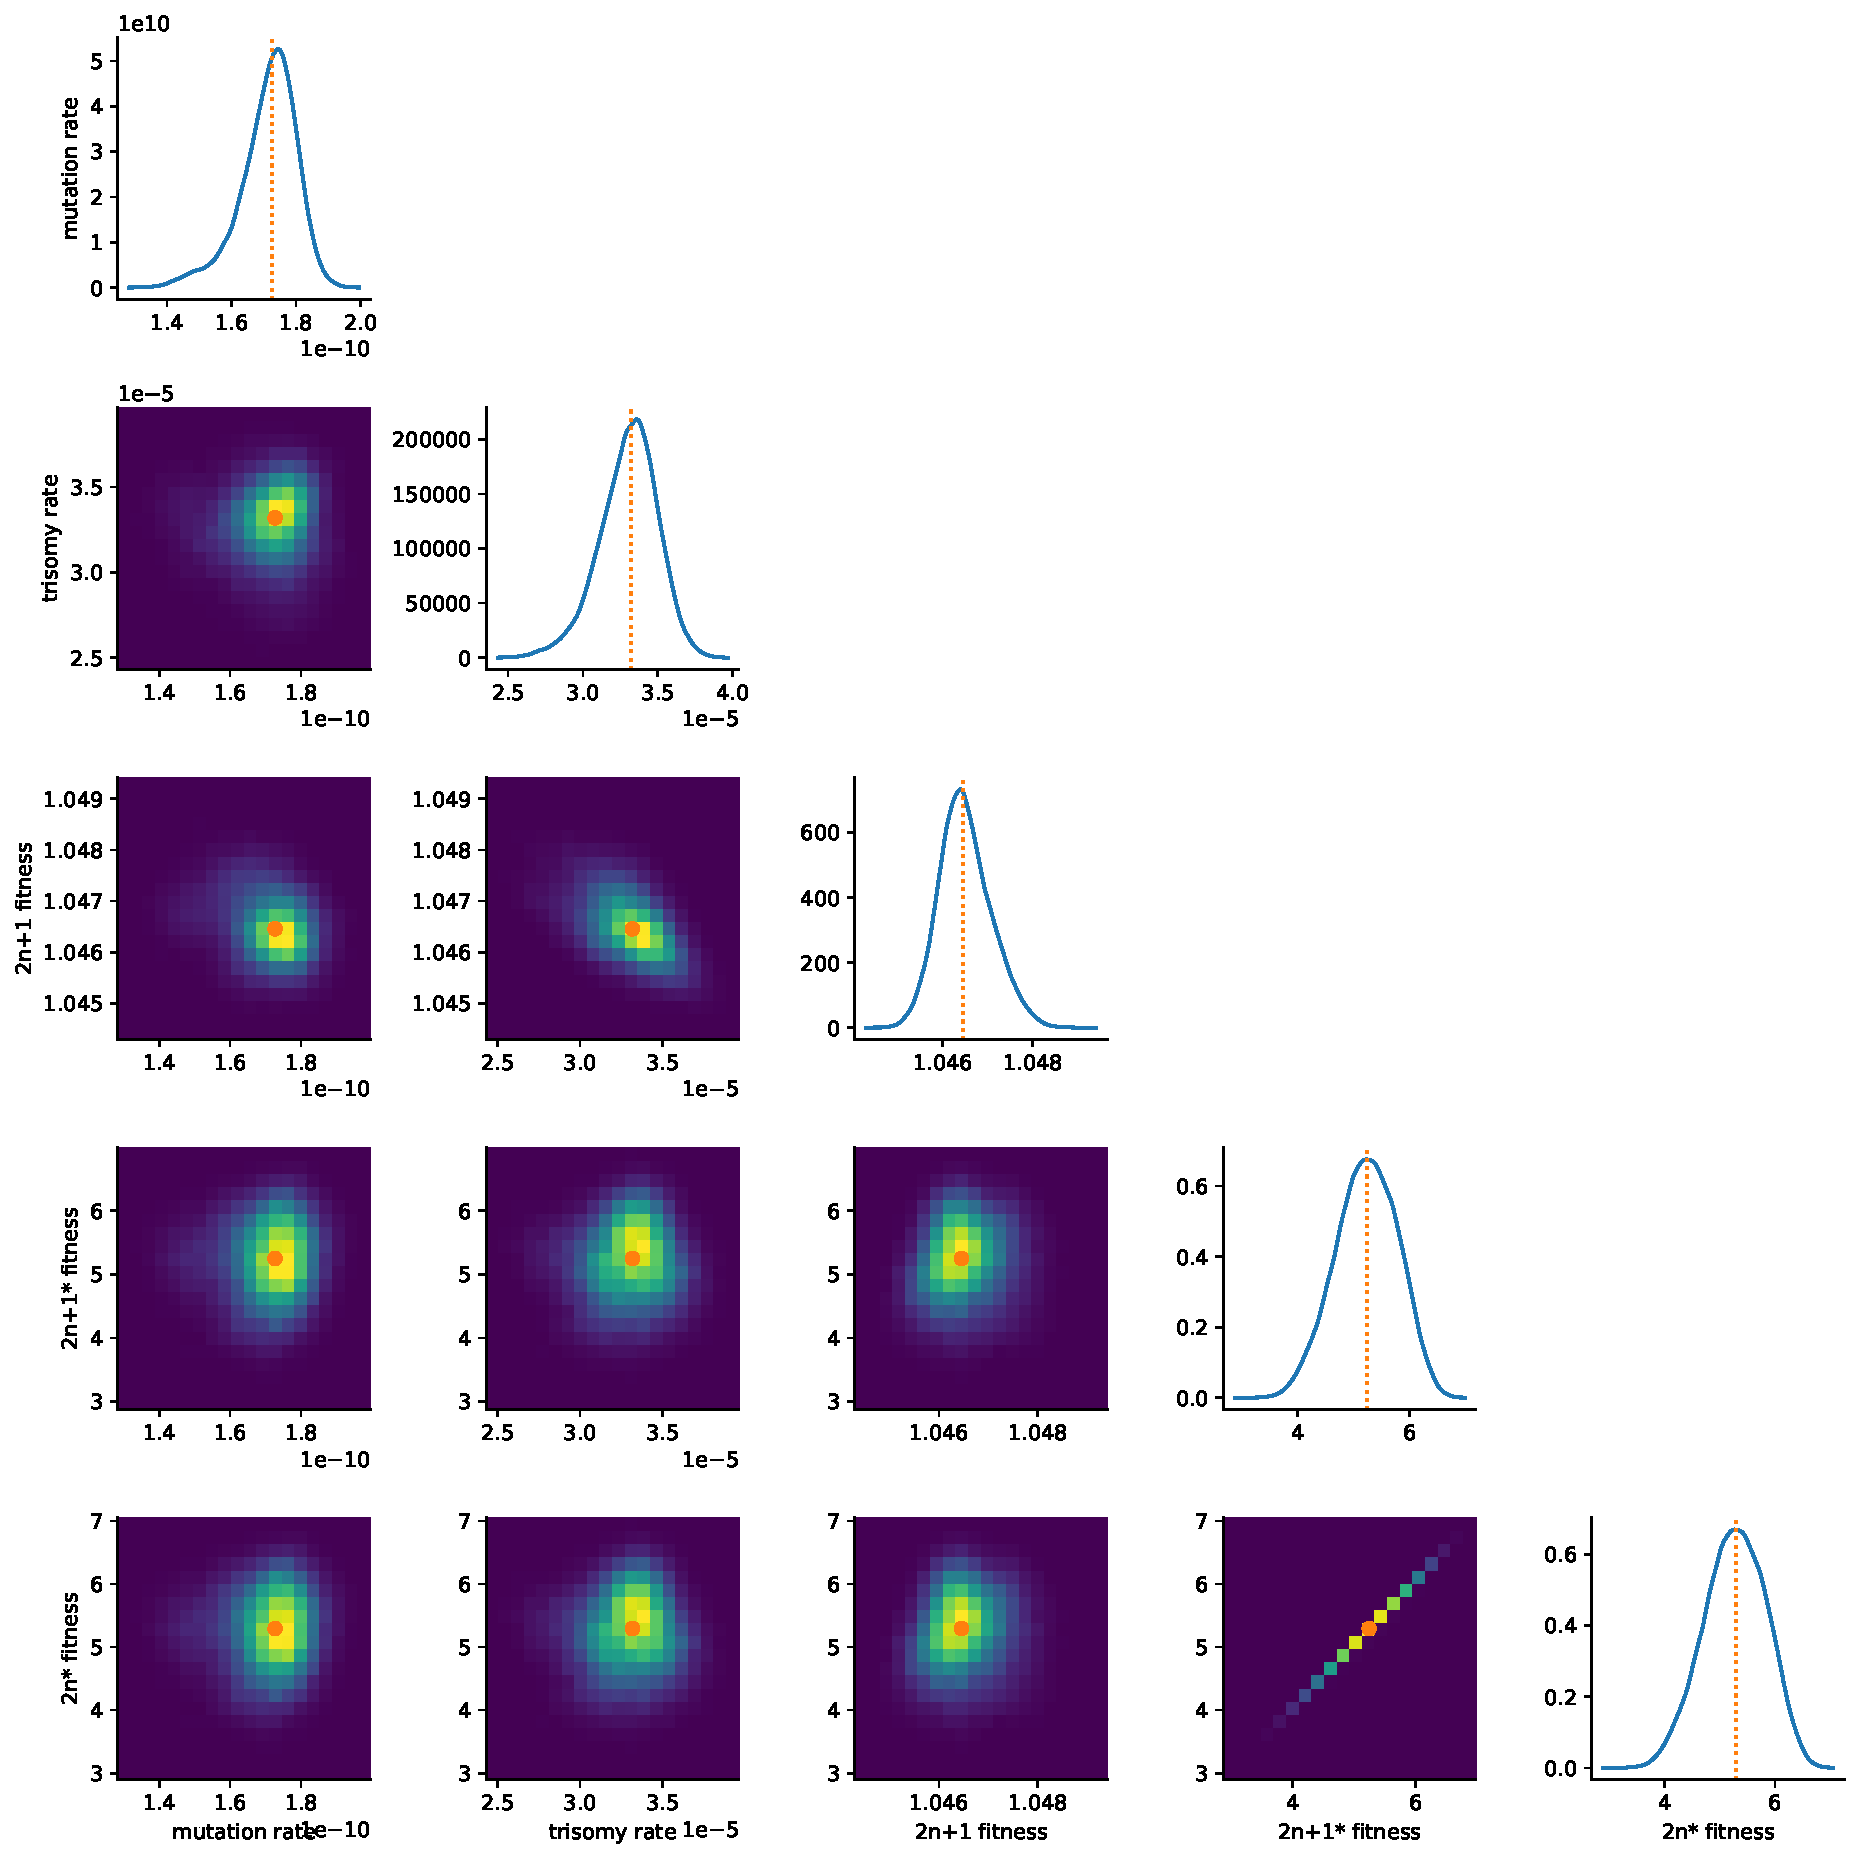
\includegraphics[width=0.9\textwidth]{../figures/posterior.pdf}
  \caption{
  \textbf{Posterior distribution of model parameters.}
On the diagonal, the inferred posterior distribution of each model parameter. 
Below the diagonal, the inferred joint posterior distribution of pairs of model parameters (dark purple and bright yellow for low and high density, respectively). Red markers and orange lines for the joint MAP estimate (which may differ from the marginal MAP, as the marginal distribution integrates over all other parameters).
} 
  \label{fig:posterior}
\end{figure}
%%%%%%%%%%%%%%%%%%%%%%

\paragraph{Model checking and comparison.}
The model fits the data well: in simulations using the MAP parameter estimates, \eumt\ fixed in 61\% of simulations by generation 1,700 and in 100\% of simulations by generation 2,350~(\Cref{fig:2n*-fixation}B). 
Interestingly, the genotype frequency dynamics in these simulations demonstrate that \anmt\ never reaches substantial frequency (\Cref{fig:ppc-plot}).

Moreover, a model without aneuploidy (where the aneuploidy rate is fixed at zero, $\delta=0$), fails to explain the experimental observations~(Figure~\ref{fig:2n*-fixation}). %% generated with MAP-and-hdi.ipynb
The estimated mutation rate without aneuploidy is $\mu=7.979\cdot10^{-9}\ [7.903\cdot 10^{-9}-8.135\cdot10^{-9}]$, much lower compared to a model with aneuploidy and suggesting a target size of just 40. 
The fitness of the mutant is also much lower at $w_{\eumt}=1.013\ [1.012-1.013]$.
This is because, without aneuploidy, a high mutation rate or fitness effect will lead to faster appearance and fixation of \eumt\ than in the experimental observations. Even with these lower estimates, the model fit is worse than that of a model with aneuploidy~(\Cref{fig:2n*-fixation}). 

% Rancati G, Pavelka N. Karyotypic changes as drivers and catalyzers of cellular evolvability: A perspective from non-pathogenic yeasts. Semin Cell Dev Biol. 2013;24(4):332-338. doi:10.1016/j.semcdb.2013.01.009
% Bouchonville K, Forche A, Tang KES, Semple C a M, Berman J. Aneuploid chromosomes are highly unstable during DNA transformation of Candida albicans. Eukaryot Cell. 2009;8(10):1554-1566. doi:10.1128/EC.00209-09
% Zhu J, Pavelka N, Bradford WD, Rancati G, Li R. Karyotypic determinants of chromosome instability in aneuploid budding yeast. PLoS Genet. 2012;8(5). doi:10.1371/journal.pgen.1002719

It has been suggested that aneuploidy increased genetic instability~\citep{Sheltzer2011b}. Therefore, we inferred model parameters under the assumption that the mutation rate increases in aneuploid cells by a factor $\tau$ = 33/32 (due to an additional chromosome), 2, 5, 10, or 100 (due to genetic instability).
We found that the posterior distribution was similar for $\tau=$1, 33/32, 2, and 5 (\Cref{fig:tau}).
%% generated with MAP-and-hdi.ipynb
With $\tau=100$, the estimated mutation rate was about 7-8-fold lower compared to $\tau=1$ ($\mu=3.81\cdot10^{-7}\ [1.508\cdot10^{-7}-4.995\cdot10^{-7}]$) and the aneuploidy rate was about 2-3-fold lower ($\delta=0.782\cdot10^{-3}\ [0.661\cdot10^{-3}-1.462\cdot10^{-3}]$). 
With $\tau=10$, the estimated mutation rate was only slightly lower compared to $\tau=1$ ($\mu=1.674\cdot10^{-6}\ [2.501\cdot10^{-7}-1.741\cdot10^{-6}]$). 
WAIC is lowest for $\tau=100$~(\Cref{table:WAIC}), and if we rule such a strong effect of genetic instability a-priori, the next two lowest WAIC values are for $\tau=33/32$ and $\tau=5$.  
Therefore, we cannot rule out an increased mutation rate in aneuploid cells, but unless the effect is strong ($\tau=100$), it does not seem to affect our inference results.
We also checked the differences in fixation/loss times of  \euwt, \anwt and \eumt\  for the models with different $\tau$. We saw that the models can be distinguished using these parameters, especially $\tau=100$~(\Cref{fig:tau-plots}).

Sensitivity analysis shows that changing a single parameter while keeping the rest fixed at the MAP estimate produces a worse fit to the data~(\Cref{fig:sensitivity}).
Furthermore, we fitted models with a mutation rate fixed at $\mu$=$10^{-5}$, $10^{-6}$ and $10^{-7}$. We inferred similar parameters estimates for the model with $\mu=10^{-6}$ compared to the model with a free $\mu$ parameter. Models with $\mu$=$10^{-5}$ and $\mu$=$10^{-7}$ inferred different parameters estimates~(\Cref{fig:mu}).
WAIC was lower when $\mu$ is fixed~(\Cref{table:WAIC}), but this is not surprising, as WAIC attempt to balance between model fit and model complexity, where the latter takes into account the number of model parameters. 

% generated with alt-prior.ipynb
Finally, we estimated the parameters under an extended informative prior (see \emph{Prior distributions}), with more informed priors for $w_{\anmt}$ and $w_{\eumt}$.
The posterior predictive plot show that inference with this extended prior produces a posterior distribution that fails to explain the empirical observations~(Figure~\ref{fig:2n*-fixation}).
Despite this, it produces a lower WAIC, $-57$ compared to $295$ with our standard prior, as the inferred posterior distribution is considerably narrower (compare \Cref{fig:posterior,fig:posterior-alt}), which greatly affects WAIC due to its dependence on variance (\cref{eq:WAIC}).
The estimated mutation rate was much lower compared to the previously used prior, with $\mu=2.379\cdot10^{-9}\ [2.267\cdot10^{-9}-2.458\cdot10^{-9}]$. Other parameter estimates are: $\delta=2.636\cdot10^{-3}\ [2.245\cdot10^{-3}-2.919\cdot10^{-3}]$,
$w_{\anwt}=1.022\ [1.021-1.023]$,
$w_{\anmt}=1.032\ [1.03-1.035]$,
$w_{\eumt}=1.033\ [1.031-1.036]$. 

% Fig model with and without aneuploidy
%% generated with with-aneuploidy_vs_no_aneuploidy.ipynb
\begin{figure}[p]
  \begin{subfigure}{0.5\textwidth}
      \centering
      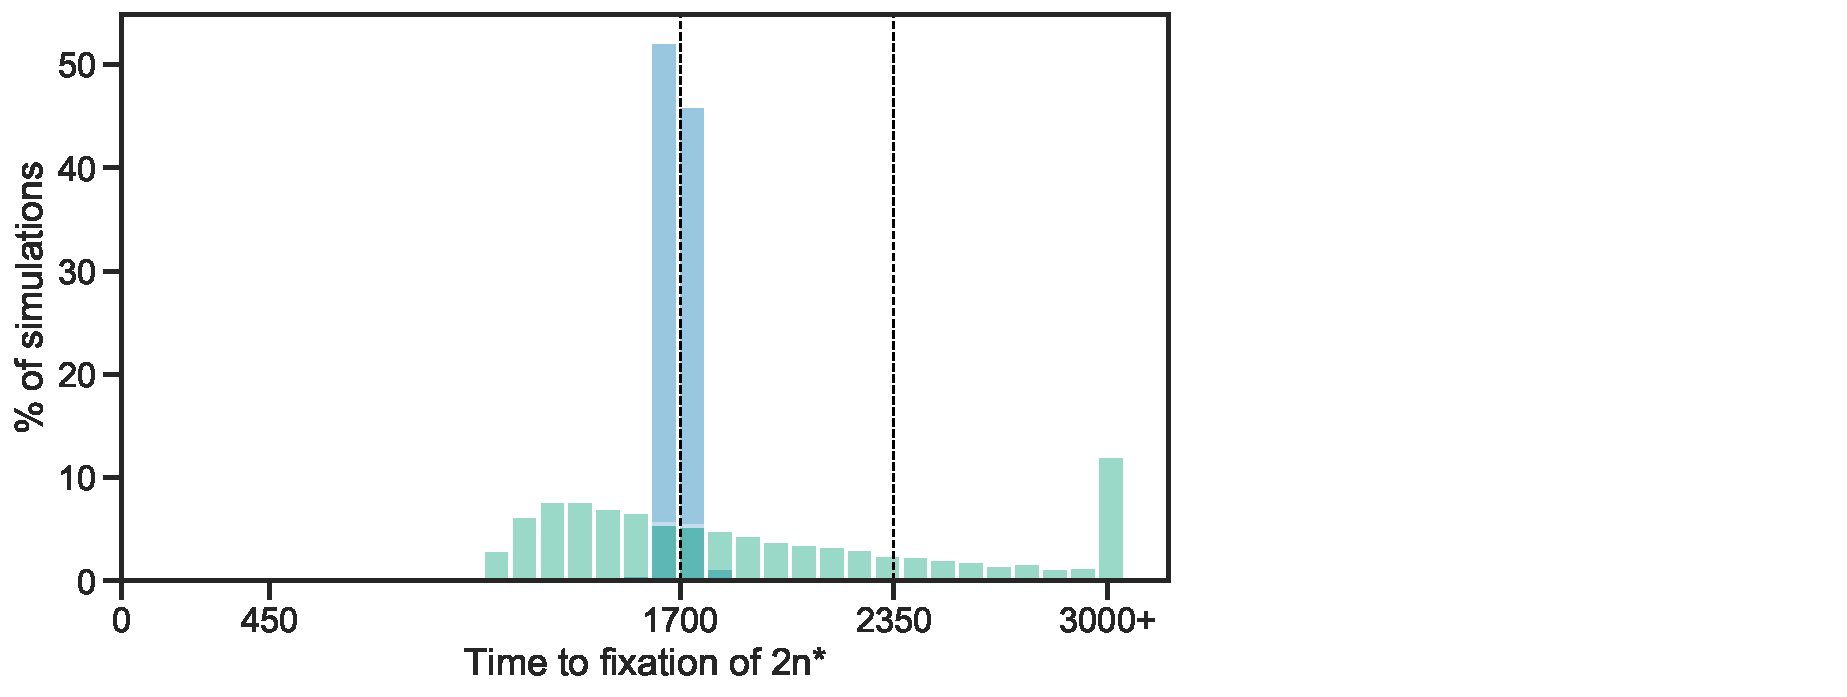
\includegraphics[width=\textwidth]{../figures/fixation-plot-a.pdf}      
      \label{fig:fit}
  \end{subfigure}
  \begin{subfigure}{0.5\textwidth}
      \centering
      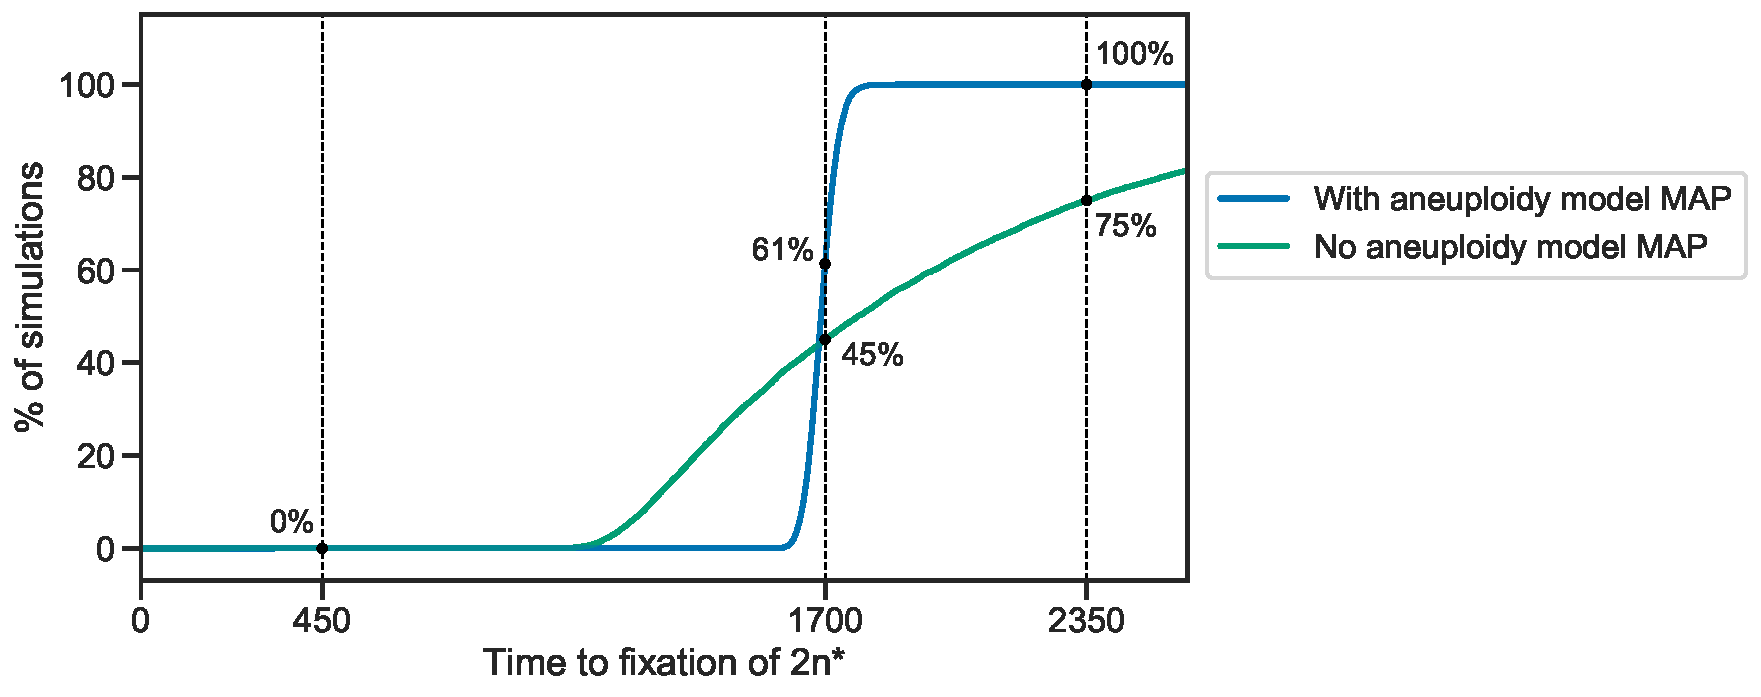
\includegraphics[width=\textwidth]{../figures/fixation-plot-b.pdf}      
      \label{fig:fit-cumulative}
  \end{subfigure}
  \caption{
    \textbf{Model fit with and without aneuploidy.}
    \textbf{(A)} The distribution of time to fixation of \eumt\ (i.e., adaptation time) in $10,000$ simulations of the model with aneuploidy (blue; MAP parameters) compared to two models without aneuploidy: a model with the same parameter values except $\delta=0$ (orange), and a model fitted to the data assuming $\delta=0$ (green); and to the model with aneuploidy with extended prior distribution (pink).
In the experiment by \citet{Yona2012}, one population lost aneuploidy by generation 1,700 and another by generation 2,350 (dashed lines) but not before generation 450. Thus, the blue distribution is a better fit compared to the green and pink, and the yellow histogram has a very poor fit.
The last bin contains all values equal or greater than 3,000.
    \textbf{(B)}
	Cumulative distribution of the time to fixation of \eumt\ in 10,000 simulations using the MAP estimate with and without aneuploidy in blue and green, respectively, and corresponding to the blue and green bars in panel A. The MAP likelihood (\cref{eq:heatstress-likelihood}) is 0.84, 0.67, and 0.14 for the models represented by blue, green, and pink distributions, respectively. 
     }
  \label{fig:2n*-fixation}
\end{figure}

\begin{figure}[p]
  \centering
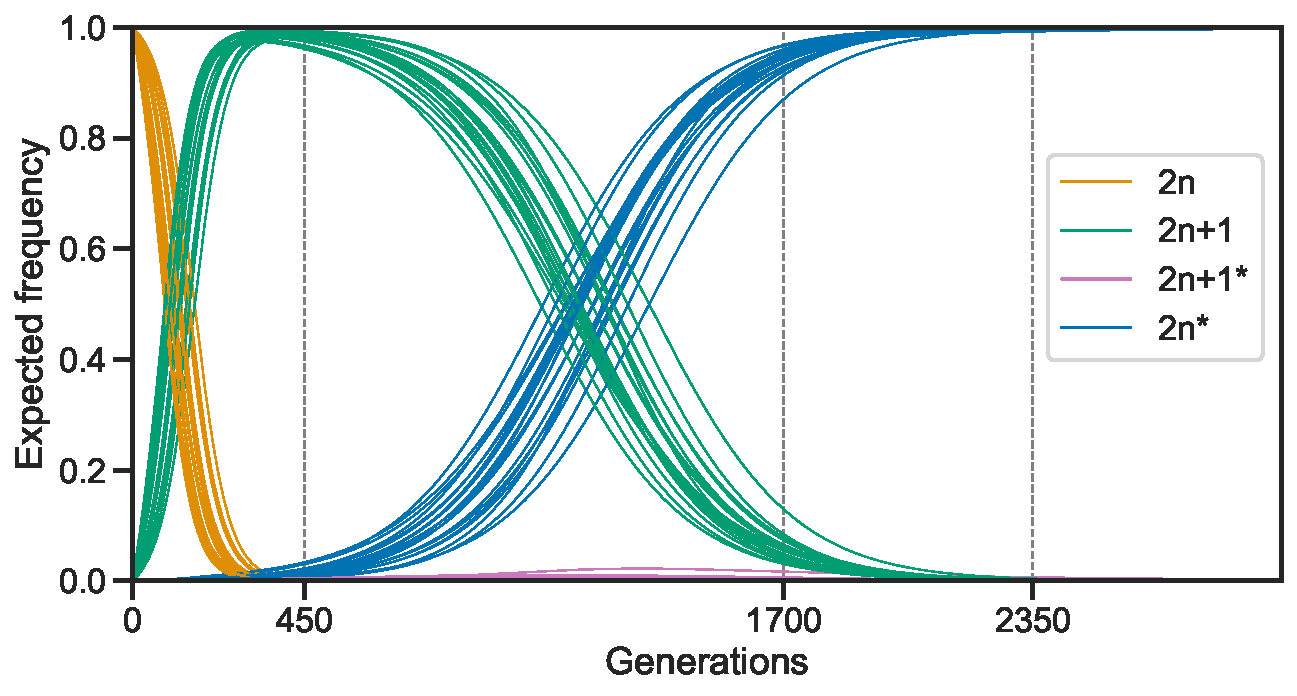
\includegraphics[width=0.8\textwidth]{../figures/dynamics.pdf}
  \caption{
  \textbf{Posterior genotype frequency dynamics for the model.} 
  The posterior prediction for the frequencies of the four genotypes over time. Each of the 20 curves is the average of 10,000 simulations of the model using parameters drawn from the posterior distribution.
  }
  \label{fig:ppc-plot}
\end{figure}

% Fig tau plots
%% generated by diff-tau-plots.ipynb
\begin{figure}[p]
  \centering
  \begin{subfigure}{0.75\textwidth}
      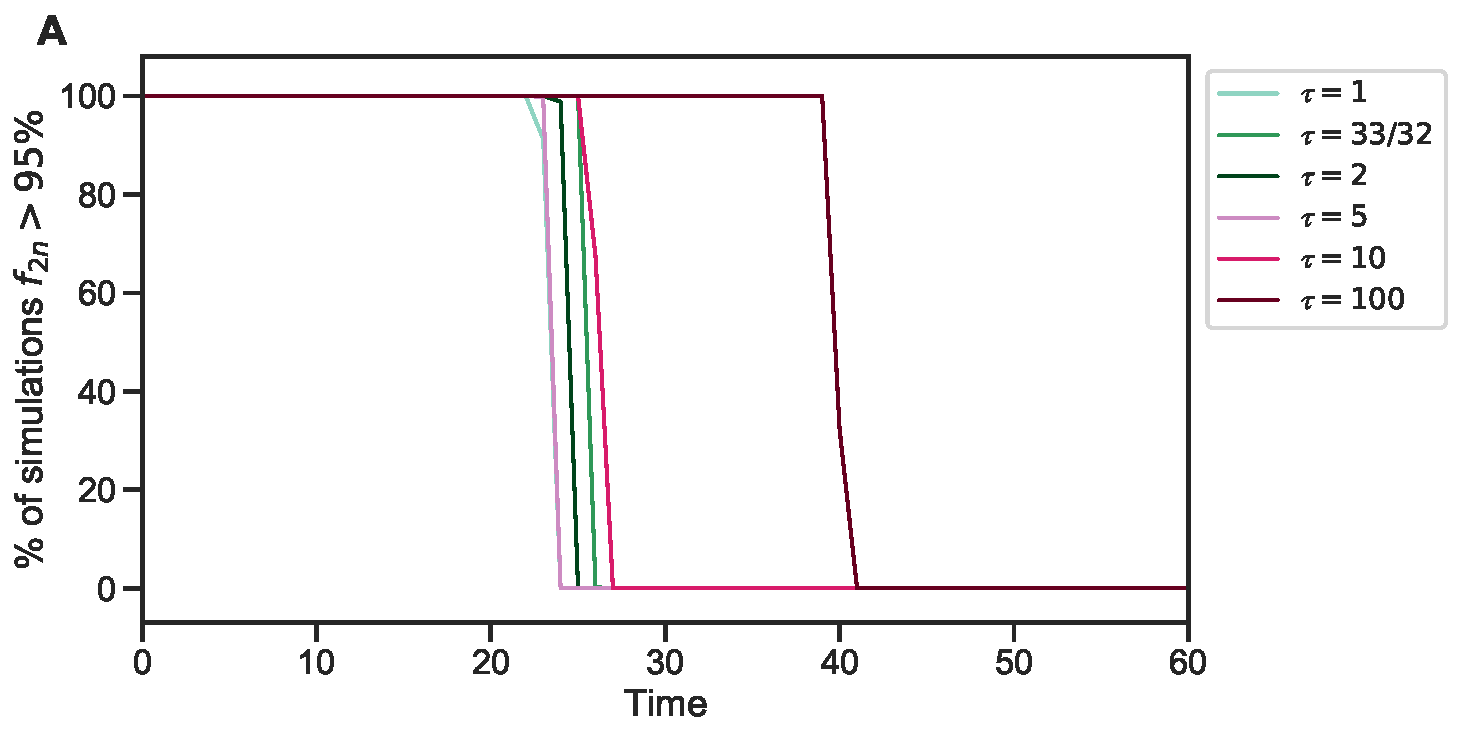
\includegraphics[width=\textwidth]{../figures/tau-diff-a.pdf}      
  \end{subfigure}
  \begin{subfigure}{0.75\textwidth}
      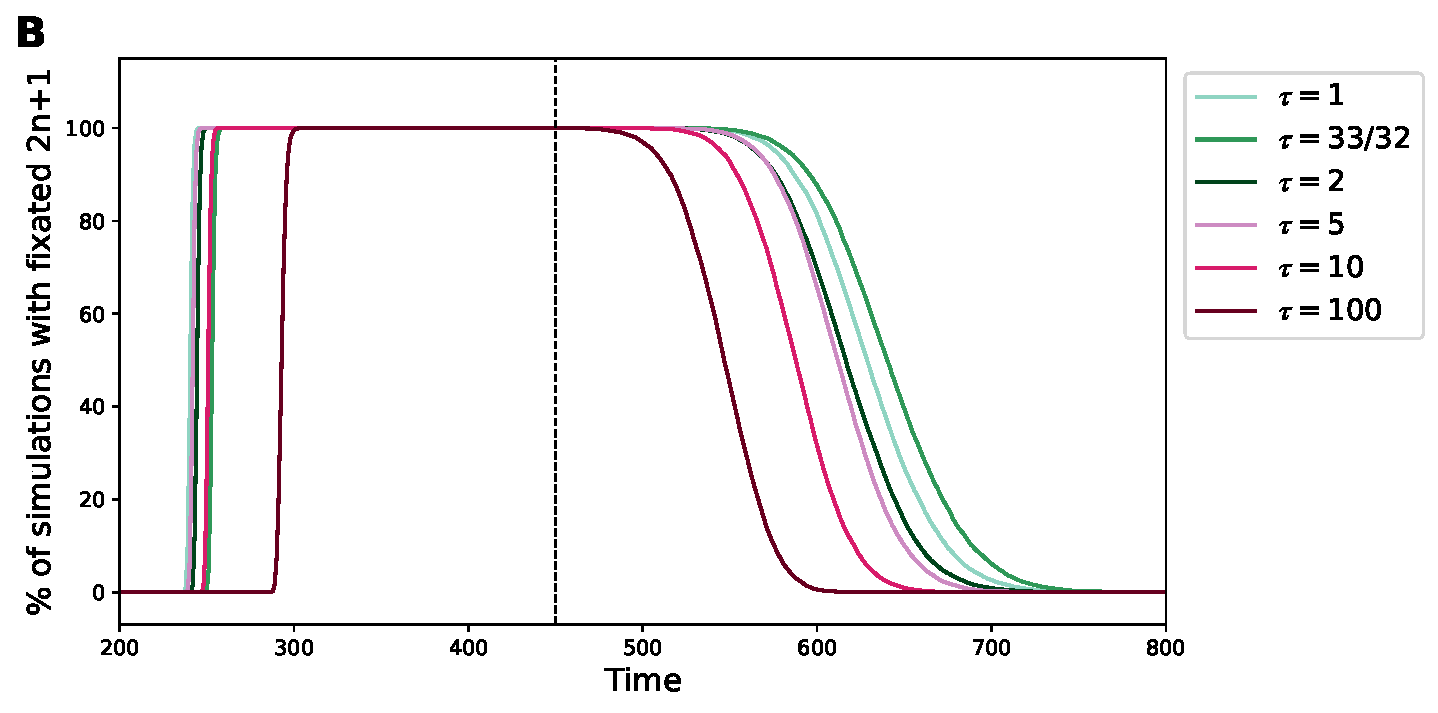
\includegraphics[width=\textwidth]{../figures/tau-diff-b.pdf}      
  \end{subfigure}
   \begin{subfigure}{0.75\textwidth}
      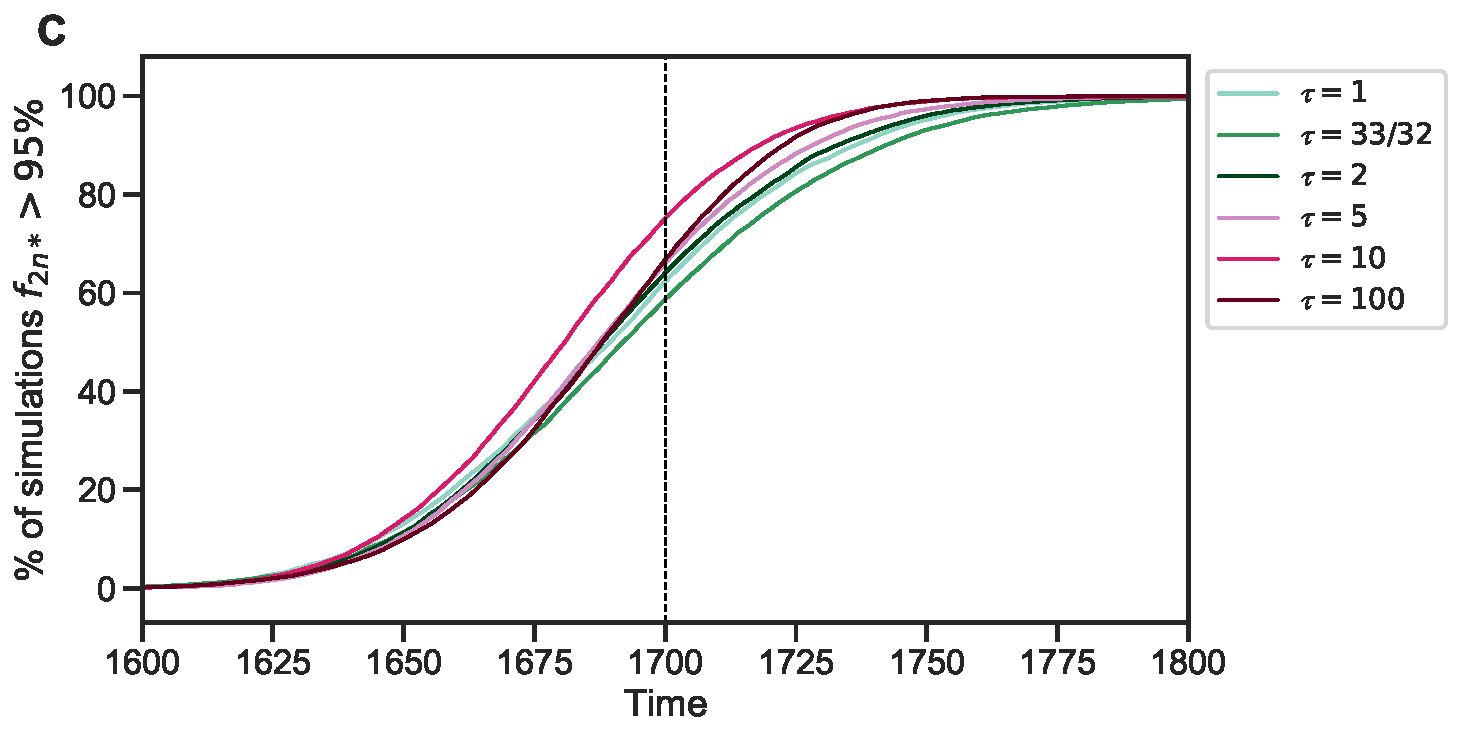
\includegraphics[width=\textwidth]{../figures/tau-diff-c.pdf}      
  \end{subfigure}
   \caption{
    \textbf{Genotype fixations for models with increased genetic instability.} We estimated the parameters for different models, each assuming a different value of $\tau$, the fold-increase in mutation rate in aneuploid cells. We then generated 10,000 simulations using the MAP estimate of each model and evaluated the fraction of simulations in which the genotype \euwt\ (\textbf{A}), \anwt\ (\textbf{B}), and \eumt\ (\textbf{C}) is fixed (y-axis) at each generation (x-axis). Note that \anmt\ did not fix. We can see that $\tau=100$ can be distinguished if time to loss of \euwt\ is known (panel~A) or if time to fixation or loss of \anwt\ is known (panel~B). It is harder to distinguish between $1\leq \tau \leq10$.
  }
  \label{fig:tau-plots}
\end{figure}


\pagebreak

%%%%%%%%%%
% Discussion
\section*{Discussion}

\paragraph*{Aneuploidy is not just another type of mutation.}
The published data indicate that, like mutation, aneuploidy can be both deleterious and beneficial~\citep{Pavelka2010, Sheltzer2011}.
Nevertheless, there are important and fundamental differences between adaptation by aneuploidy
and adaptation by beneficial mutations~\citep{Yona2015}, which make aneuploidy a unique mechanism for generating genetic
variation.
First, the aneuploidy rate (i.e. the frequency of mis-segregation events) is significantly higher than the
mutation rate~\citep{Santaguida2015review}.
Thus, everything else being equal, adaptation by aneuploidy will be faster and more frequent.
Second, fitness effects of aneuploidy are larger than those of the majority of mutations, on average, and are rarely
neutral~\citep{Pavelka2010, Yona2012, Sunshine2015}, allowing selection to quickly sort deleterious and beneficial genotypes.
Third, the number of different karyotypes is considerably smaller than the number of different genotypes, and different karyotypes are likely to have different phenotypes~\citep{Pavelka2010}.
Therefore, exploration of the phenotype space by aneuploidy requires smaller populations and a shorter time span.
Fourth, aneuploidy is a reversible state, as the rate of chromosome loss is high and the cost of aneuploidy is significant~\citep{Niwa2006}.
Indeed, aneuploidy often provides a transient solution: under short-term stress conditions, aneuploidy reverts (chromosome number returns to normal) when the stress subsides; under long-term stress conditions, aneuploidy reverts when refined solutions, generated by beneficial mutations, take over~\citep{Yona2012}.
Finally, aneuploidy results in increased genome instability, potentially increasing genetic variation by a positive feedback loop~\citep{Rancati2013, Bouchonville2009, Zhu2012}, while also increasing its own transience.

\paragraph*{Evolutionary theory of aneuploidy.}
The role of aneuploidy in adaptation has only recently been observed~\citep{Sionov2010, Yona2012, Gerstein2015}, and is largely missing from the literature on evolution and adaptation:
the introductory textbook \emph{Evolution} by~\citet{Bergstrom2012} does not mention the word aneuploidy, and the graduate-level book \emph{Mutation-Driven Evolution} by~\citet{Nei2013} only briefly mentions aneuploidy in the context of speciation, but not adaptation.
In recent reviews of the literature, aneuploidy is suggested to play an important role in fungal adaptation~\citep{Robbins2017, Todd2017} and cancer evolution~\citep{Santaguida2015review, Naylor2016, Sansregret2017}, yet these reviews cite no theoretical studies nor any quantitative models.
Indeed, evolutionary, ecological, and epidemiological studies mostly assume adaptation occurs via beneficial mutations, recombination, and sex.
Therefore, there is a critical need to develop an evolutionary theory of aneuploidy like the evolutionary theories of other mechanisms for generation of genetic variation, e.g. mutation~\citep{Lynch2010}, recombination~\citep{Hartfield2012}, and sex~\citep{Otto2009}.
An evolutionary theory of aneuploidy will be central to the interpretation of experimental and clinical observations and design of new hypotheses, experiments, and treatments~\citep{Carja2014}.
For example, despite the lack of theoretical models, aneuploidy has been invoked in a new strategy to combat pathogens and tumour cells by setting ``evolutionary traps''~\citep{Gerstein2015,Chen2015}, in which a condition that predictably leads to emergence of aneuploidy is applied, followed by a condition that specifically selects against aneuploid cells.

\pagebreak
% Acknowledgements
{\small
\section*{Acknowledgements}
We thank Yitzhak Pilpel, Orna Dahan, Lilach Hadany, Judith Berman, David Gresham, Shay Covo, Martin Kupiec, and Tal Simon for discussions and comments.
This work was supported in part by 
the Israel Science Foundation (YR 552/19) and
Minerva Stiftung Center for Lab Evolution (YR).
% TODO add Minerva for Martin; funding for Avihu?
}

\bibliographystyle{agsm}
\bibliography{ms.bib}

\newpage

\section*{Supplementary Material}
\beginsupplement % https://support.authorea.com/en-us/article/how-to-create-an-appendix-section-or-supplementary-information-1g25i5a/

% Fig Curveball 
\begin{figure}[h]
	\centering
	% generated with growth_curves.ipynb and deg = '39' 
	\includegraphics[width=.95\textwidth]{../figures/evo39_fitness_39deg.pdf} 
	% generated with growth_curves_refined.ipynb
	\includegraphics[width=0.95\textwidth]{../figures/refined_vs_evo39_fitness_39deg.pdf}
\caption{
    \textbf{Fitness estimation from growth curves.}
    \textbf{(A-D)} Fitness estimation from growth curves of \euwt\ and \anwt\ at \SI{39}{\celsius}. $\hat w_{\anwt}/w_{\euwt}$=1.024 (95\% CI: 0.959 - 1.115). \texttt{Curveball} 
    \textbf{(E-H)} Fitness estimation from growth curves of \anwt\ and \eumt\ at \SI{39}{\celsius}. $\hat w_{\eumt}/w_{\anwt}$=1.033 (95\% CI: 1.027 - 1.041).
    Growth curves previously described in \citet[Figs. 3C, 4A, and S2]{Yona2012}.
	Fitness estimated from growth curves using \texttt{Curveball}, a method for predicting results of competition experiments from growth curve data~\citep[\href{https://curveball.yoavram.com}{curveball.yoavram.com}]{Ram2019}. See \emph{Models and Methods, Prior distributions} for more details.  \textbf{(A,B;E,F)} Mono-culture growth curve data (markers) and best-fit growth models (lines).
\textbf{(C,G)} The mixed-culture prediction for the strains from A,B and E,F respectively, 6,375 generated curves. \textbf{(D,H)} The relative fitness distribution for \anwt\ relative to \euwt\ (panel D) and \eumt\ relative to \anwt\ (panel H). Figures generated by \texttt{Curveball}.
} 
\label{fig:growth-curves}
\end{figure}

% FIG posterior alt-prior
%% generated with alt-prior.ipynb
\begin{figure}[p]
  \centering
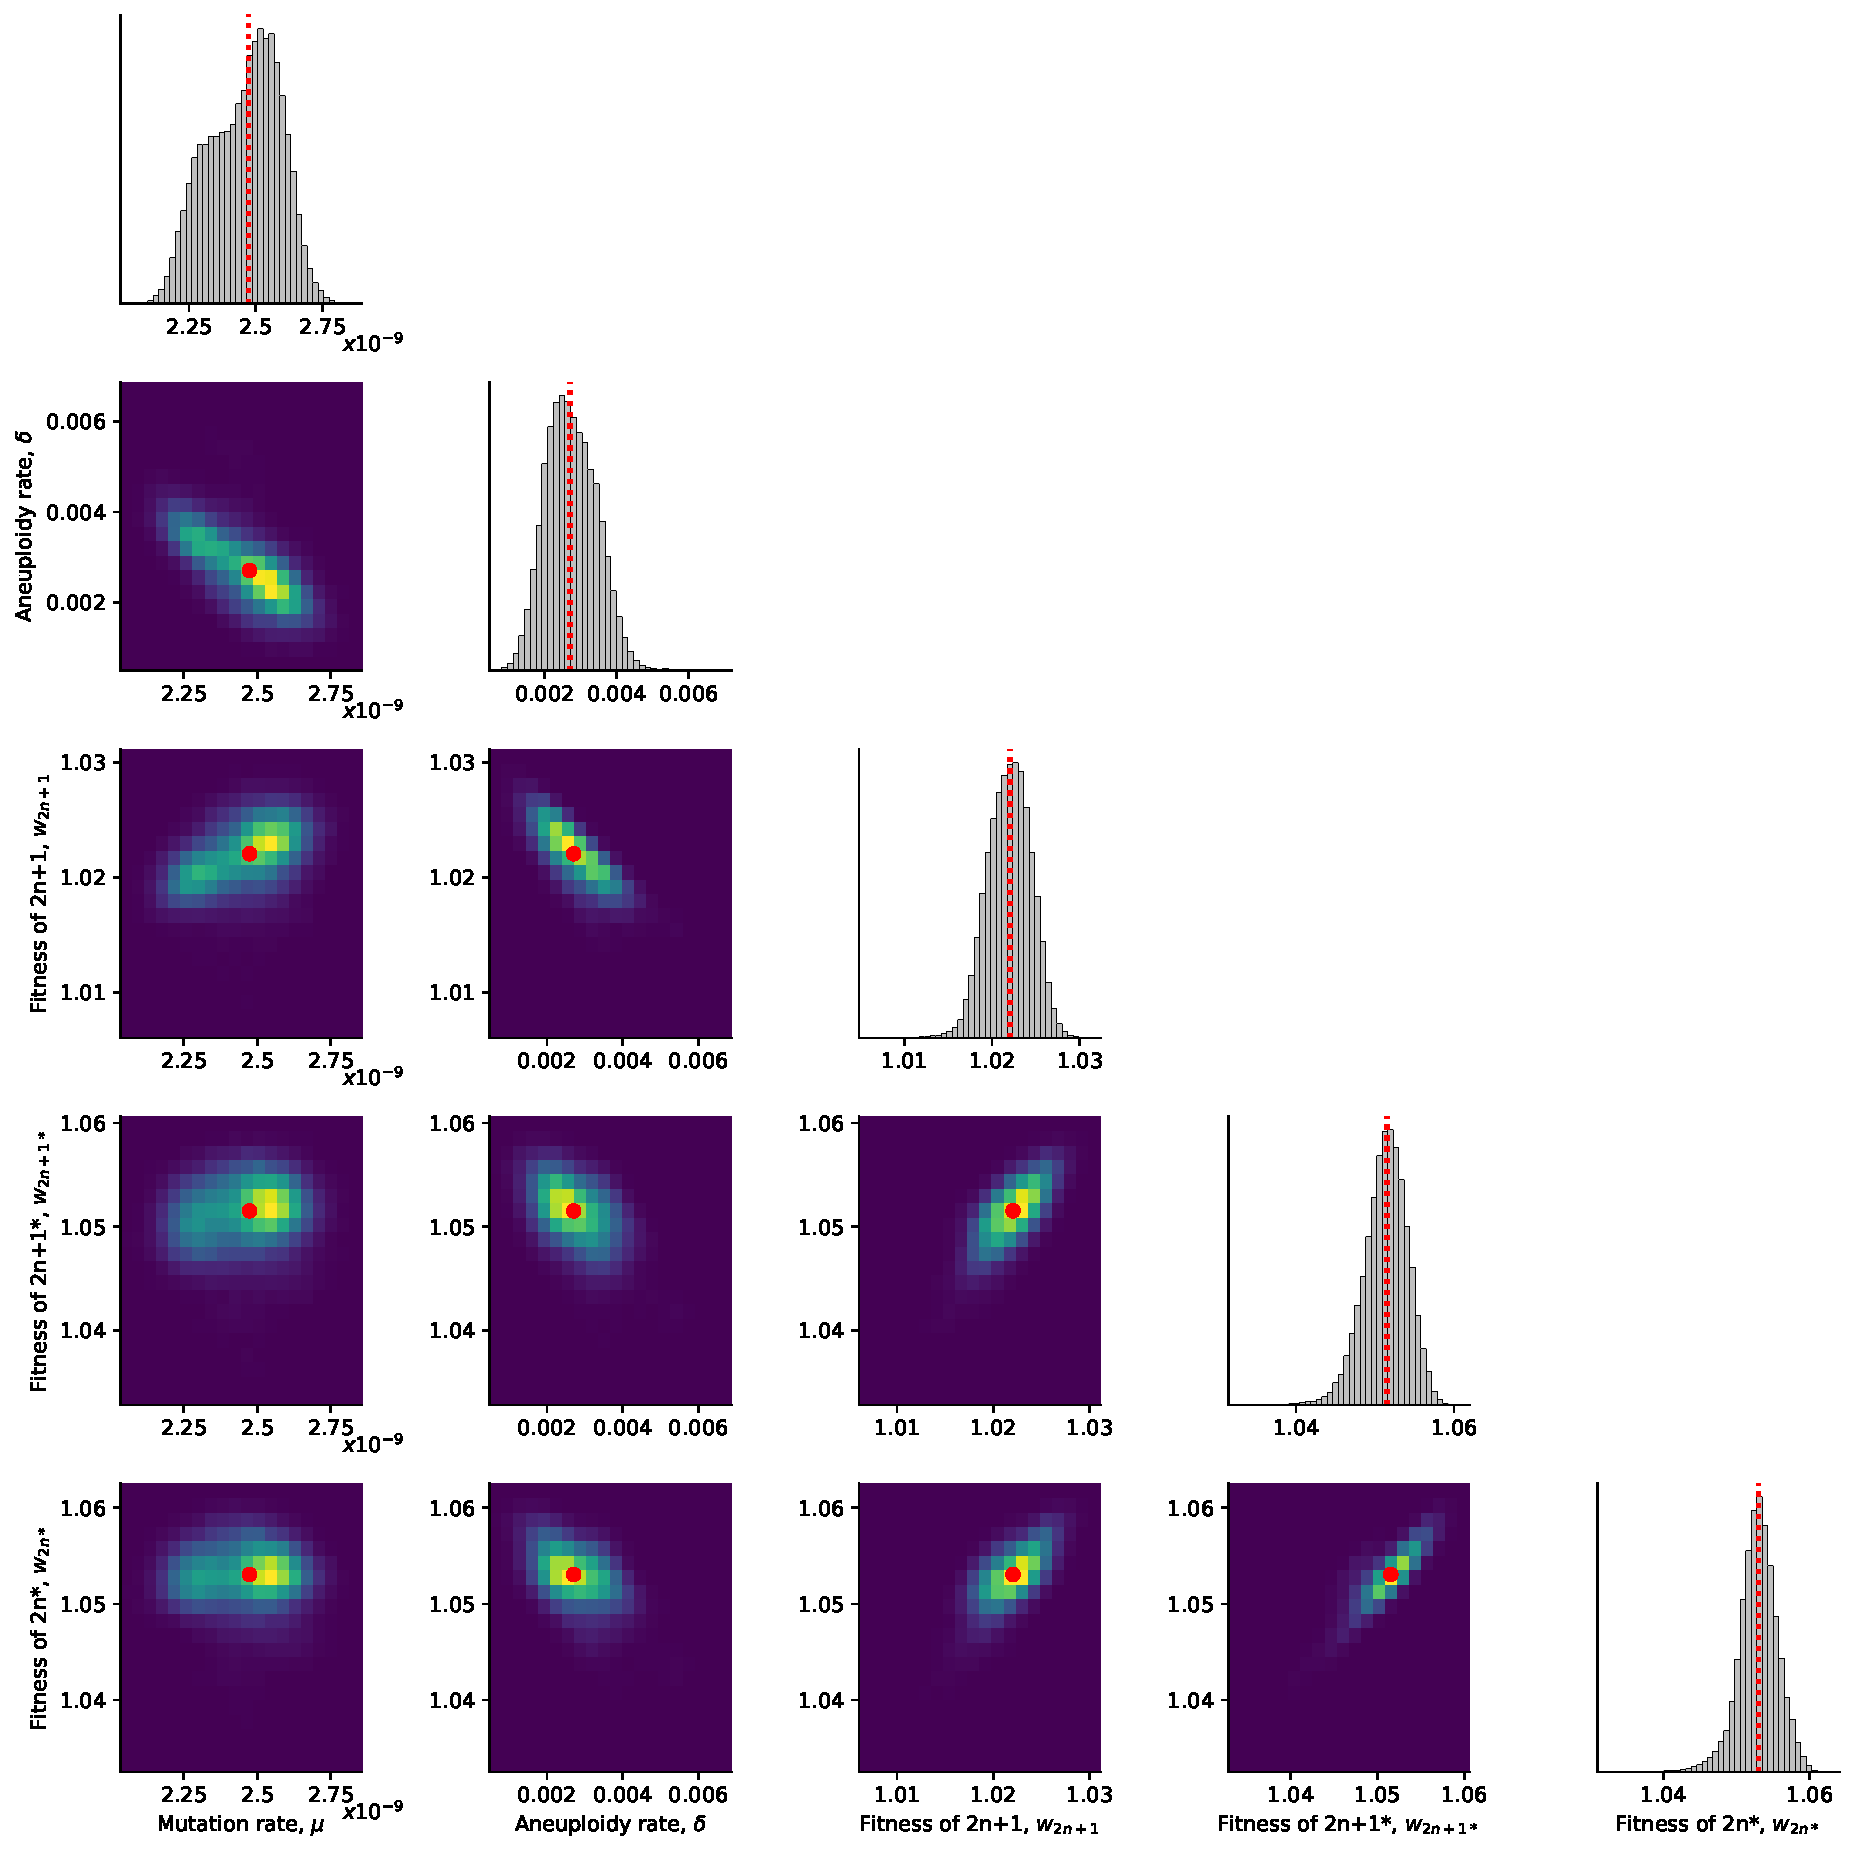
\includegraphics[width=0.9\textwidth]{../figures/posterior-alt.pdf}
  \caption{
  \textbf{Posterior distribution of parameters inferred with the extended prior distribution.}
On the diagonal, the inferred posterior distribution of each model parameter. 
Below the diagonal, the inferred joint posterior distribution of pairs of model parameters (dark purple and bright yellow for low and high density, respectively). Red markers and orange lines for the joint MAP estimate (which may differ from the marginal MAP, as the marginal distribution integrates over all other parameters).
} 
  \label{fig:posterior-alt}
\end{figure}

% Fig likelihood profile
%% generated by sensitivity-analysis.ipynb
\begin{figure}[p]
  \centering
  \begin{subfigure}{0.3\textwidth}
      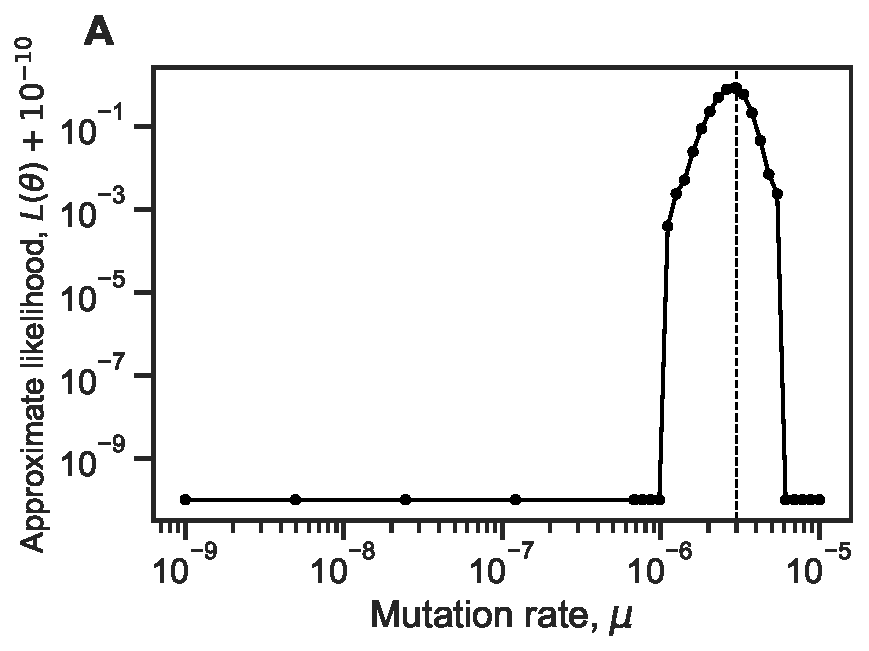
\includegraphics[width=\textwidth]{../figures/sensitivity-A.pdf}      
      \label{fig:sensitivity-mutation}
  \end{subfigure}
  \begin{subfigure}{0.3\textwidth}
      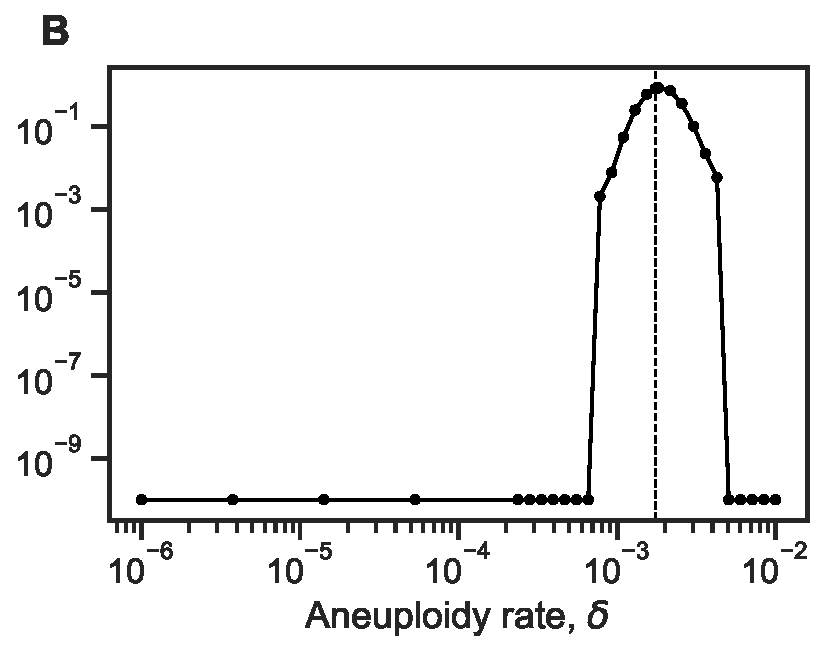
\includegraphics[width=\textwidth]{../figures/sensitivity-B.pdf}      
      \label{fig:sensitivity-aneuploidy}
  \end{subfigure}
  \\
   \begin{subfigure}{0.3\textwidth}
      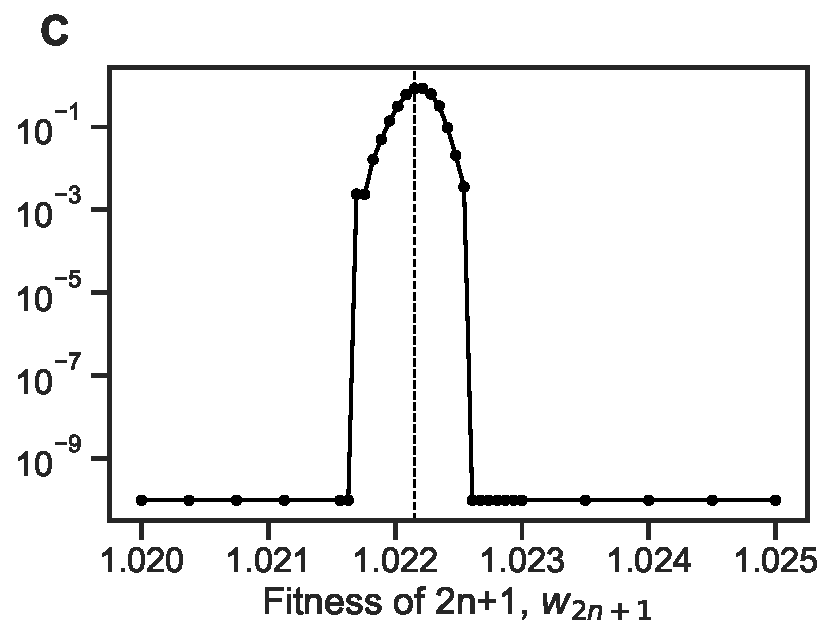
\includegraphics[width=\textwidth]{../figures/sensitivity-C.pdf}      
      \label{fig:sensitivity-anwt}
  \end{subfigure}
    \begin{subfigure}{0.3\textwidth}
      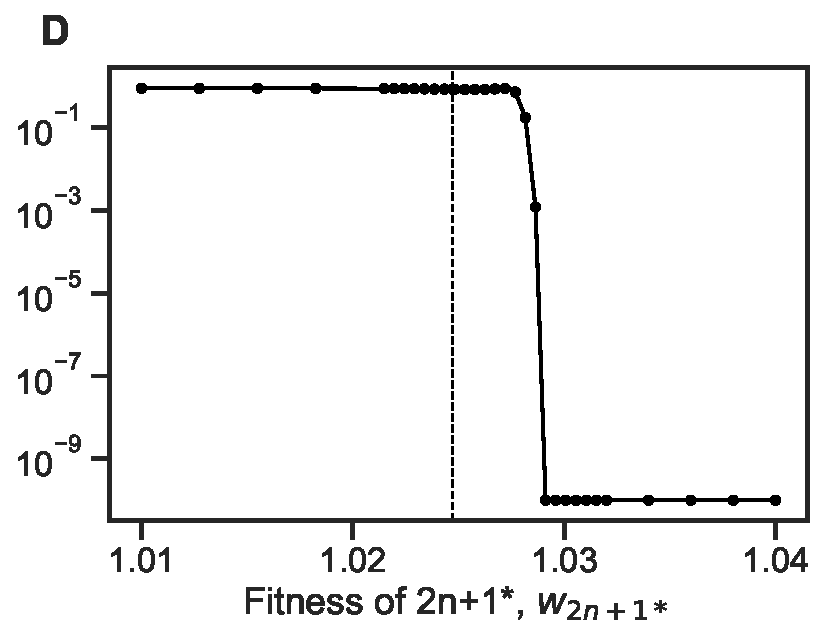
\includegraphics[width=\textwidth]{../figures/sensitivity-D.pdf}      
      \label{fig:sensitivity-anmt}
  \end{subfigure}
    \begin{subfigure}{0.3\textwidth}
      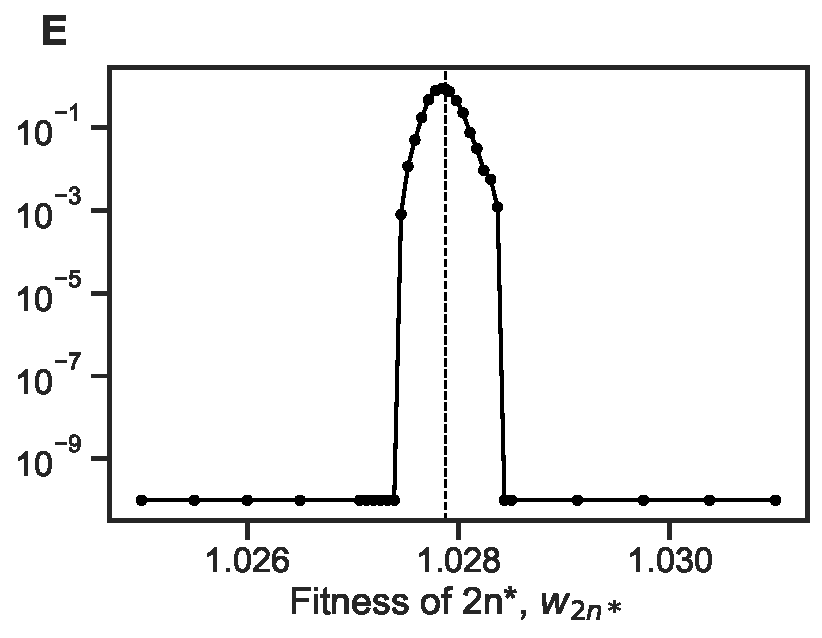
\includegraphics[width=\textwidth]{../figures/sensitivity-E.pdf}      
      \label{fig:sensitivity-eumt}
  \end{subfigure}
  \caption{
    \textbf{Likelihood profiles.} Sensitivity of the model approximate likelihood, $\likelihood(\theta)$, to changing a single parameter while the other parameters remain fixed at their MAP estimates. Dashed vertical line represents the MAP value. The prior distributions for the mutation rate and aneuploidy rate are $\mu \sim U(10^{-9}, 10^{-5})$ and $\delta \sim U(10^{-6}, 10^{-2})$, respectively. 
  }
  
  \label{fig:sensitivity}
\end{figure}


% Fig ABC iterations, convergence
%% generated with convergence.ipynb
\begin{figure}[h]

  \begin{subfigure}{1\textwidth}
    \centering
      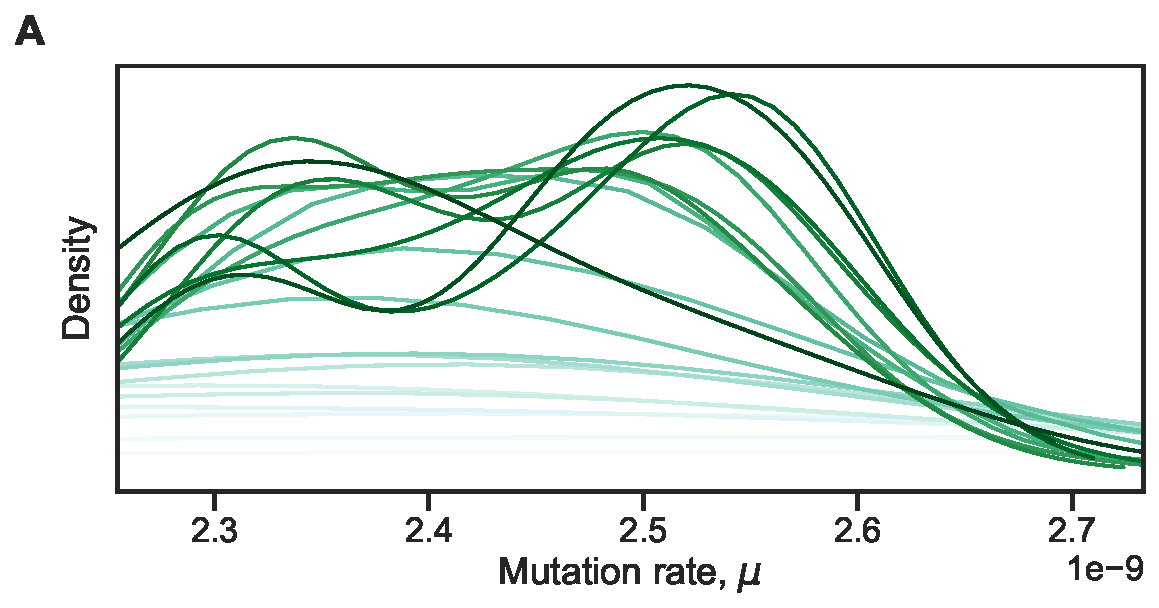
\includegraphics[width=0.45\textwidth]{../figures/convergence-p1_mr.pdf}      
      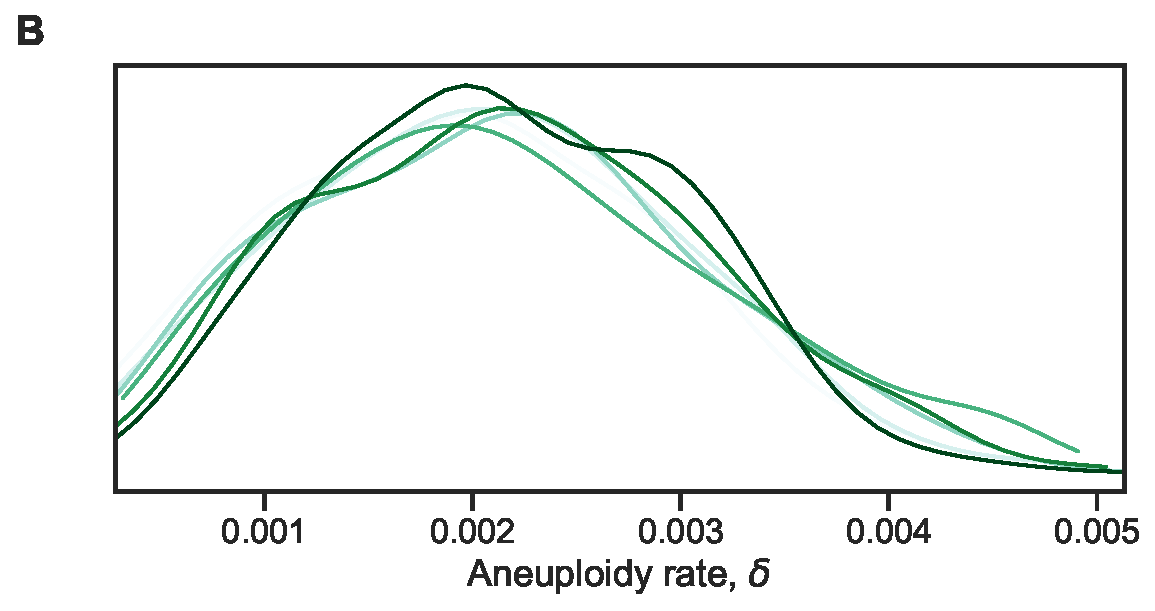
\includegraphics[width=0.45\textwidth]{../figures/convergence-p2_tr.pdf} \\     
      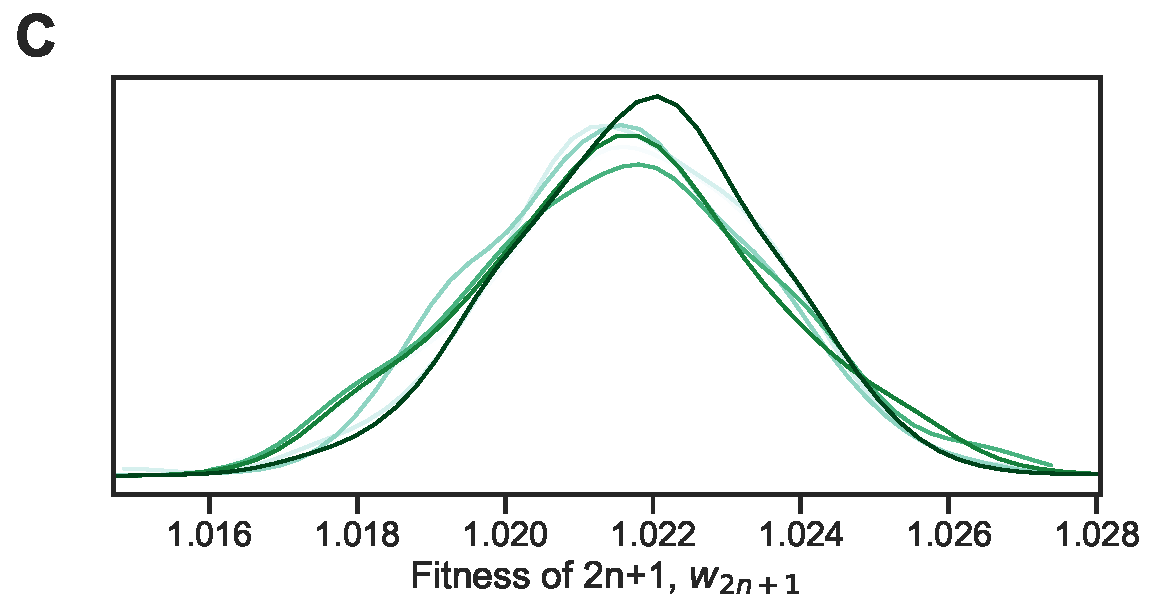
\includegraphics[width=0.325\textwidth]{../figures/convergence-p3_w1.pdf}      
      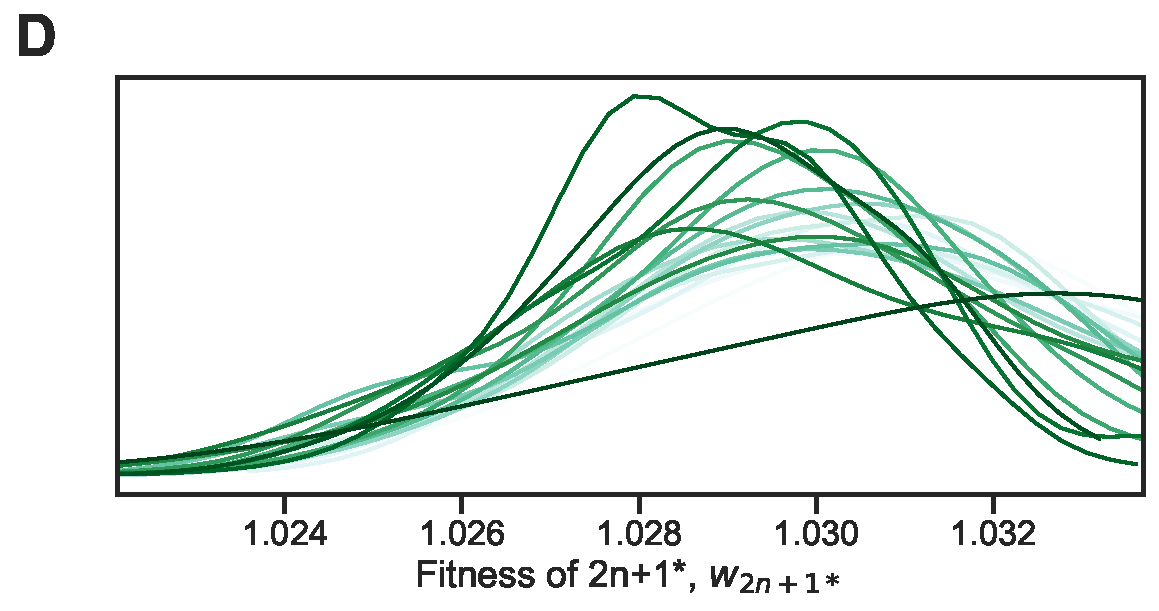
\includegraphics[width=0.325\textwidth]{../figures/convergence-p4_w2.pdf}      
      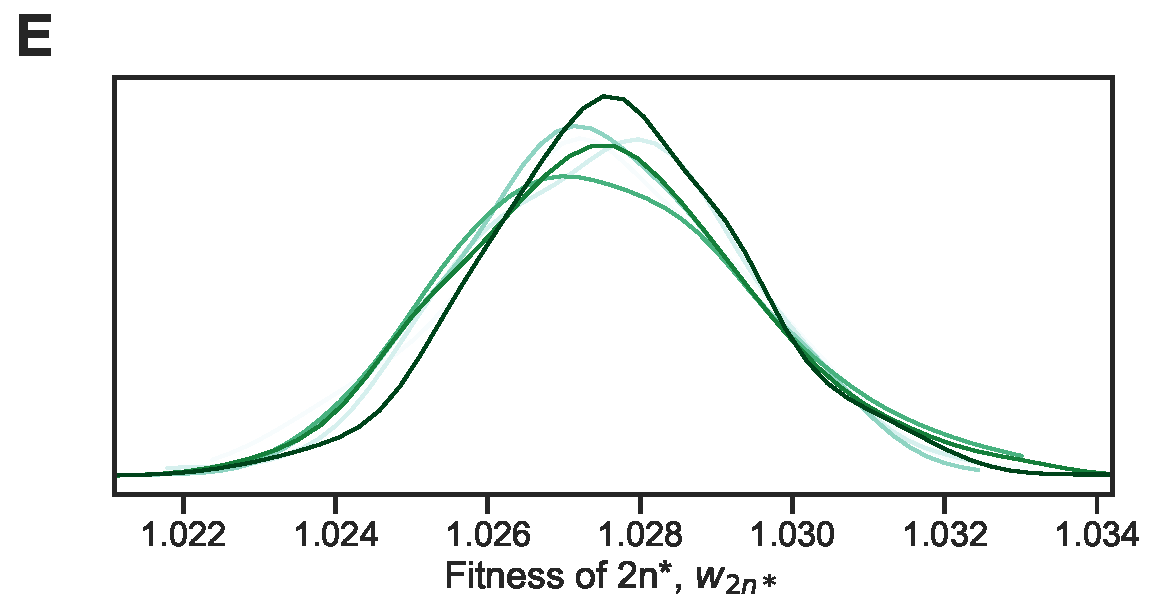
\includegraphics[width=0.325\textwidth]{../figures/convergence-p5_w3.pdf}      
     \label{fig:convergence-A}
    \end{subfigure}
    \\    
  \begin{subfigure}{1\textwidth}
  	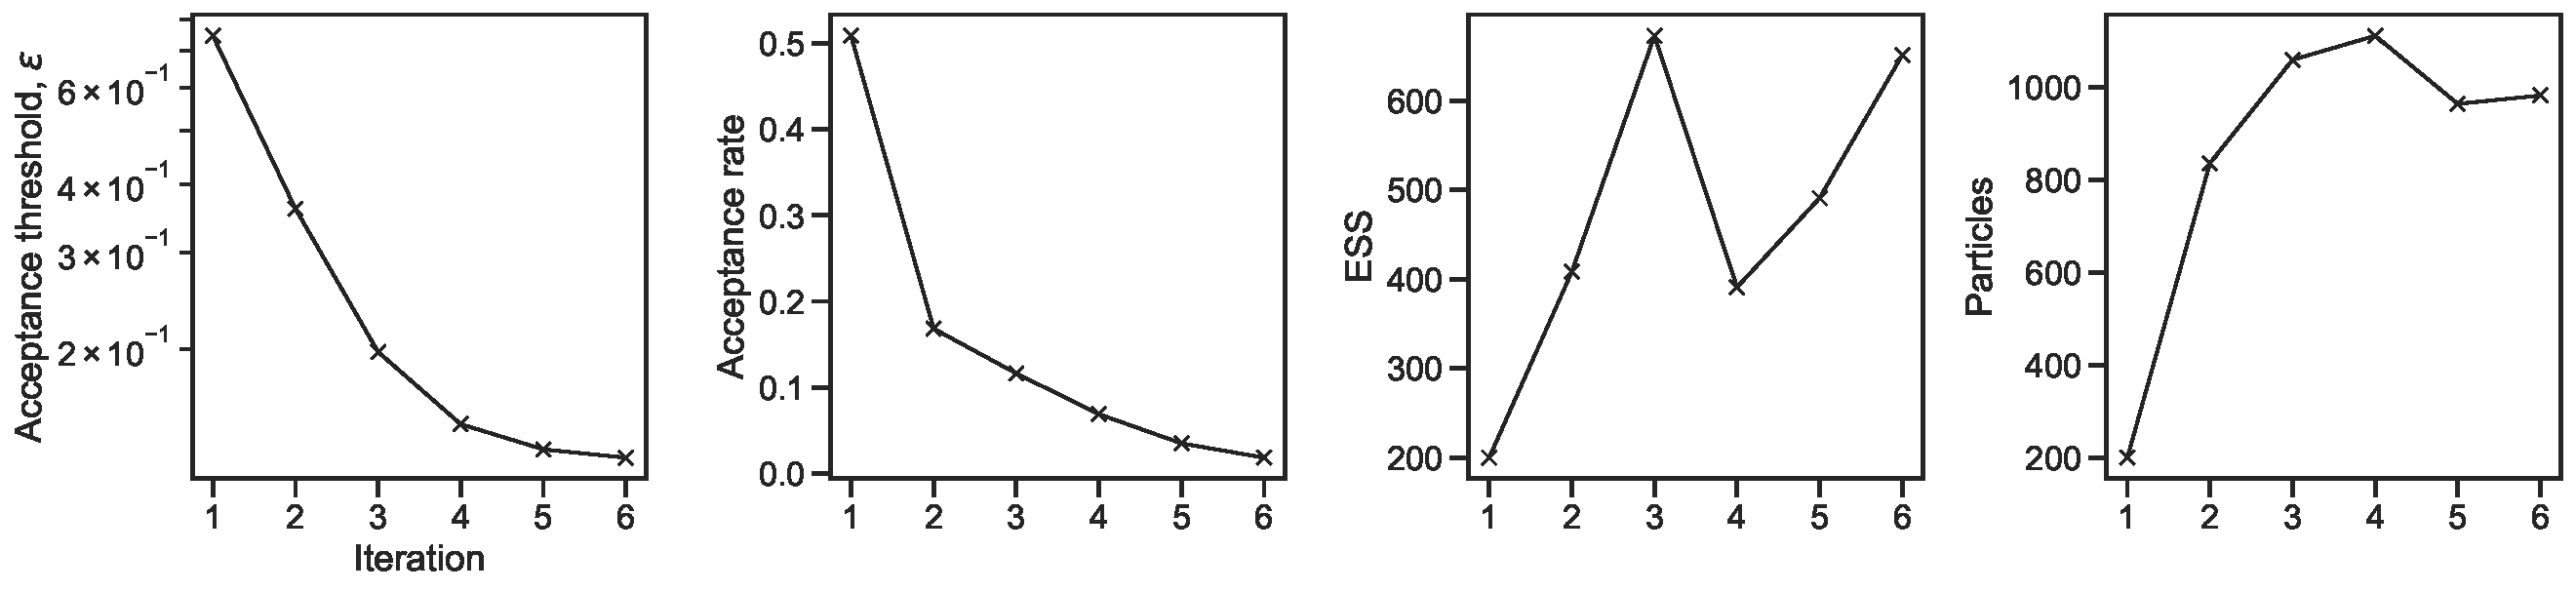
\includegraphics[width=\textwidth]{../figures/ess.pdf}
     \label{fig:convergence-B}
  \end{subfigure}
    \caption{
    \textbf{Inference convergence.} 
    The ABC-SMC algorithm was used to infer the model parameters. \textbf{(A-E)} The approximate posterior distributions of model parameters at each iteration of the ABC-SMC algorithm demonstrates convergence, as the posterior did not significantly change after the first iteration, $t=1$.
    \textbf{(F-I)} ABC-SMC measures of convergence. After iteration number 6, the acceptance threshold was $\epsilon=0.13$, the acceptance rate was $0.018$, the number of particles was 982, and the effective sample size ESS=651.
}
    \label{fig:convergence}
\end{figure}


% Fig Validation of posteriors
%% generated with diff-runs.ipynb
\begin{figure}[h]
    \centering
      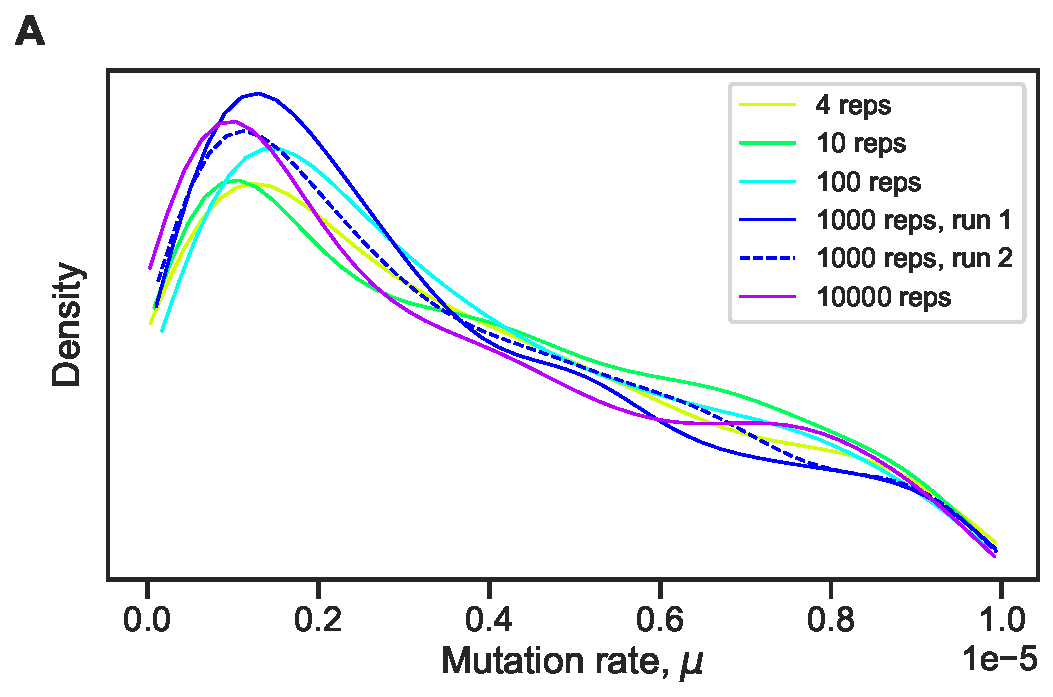
\includegraphics[width=0.45\textwidth]{../figures/runs-A.pdf}      
      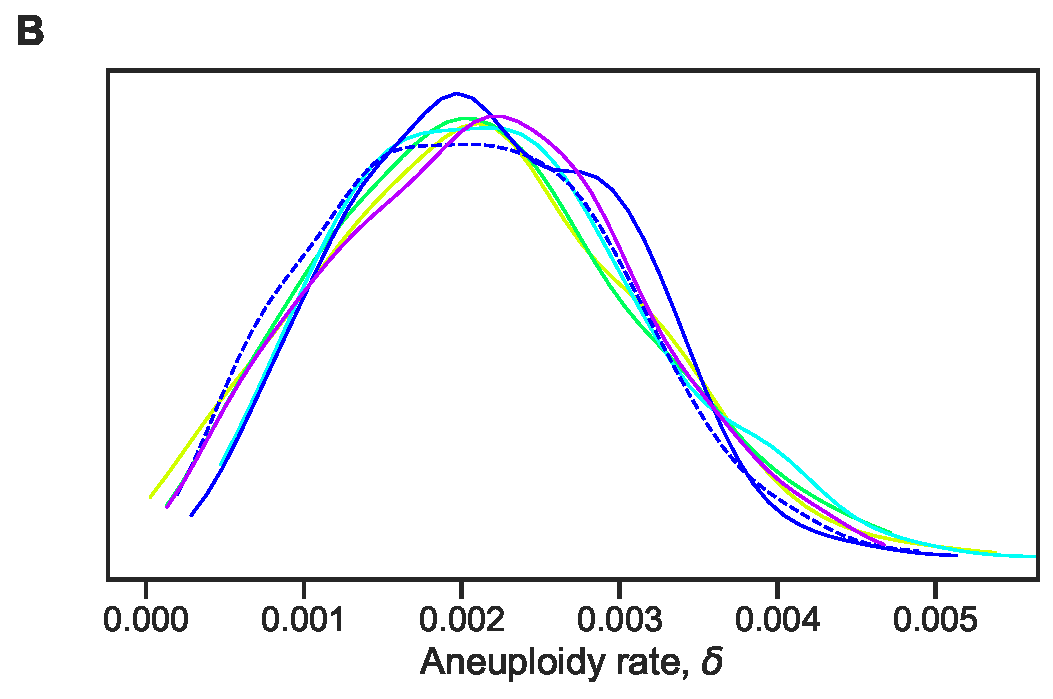
\includegraphics[width=0.45\textwidth]{../figures/runs-B.pdf}    
      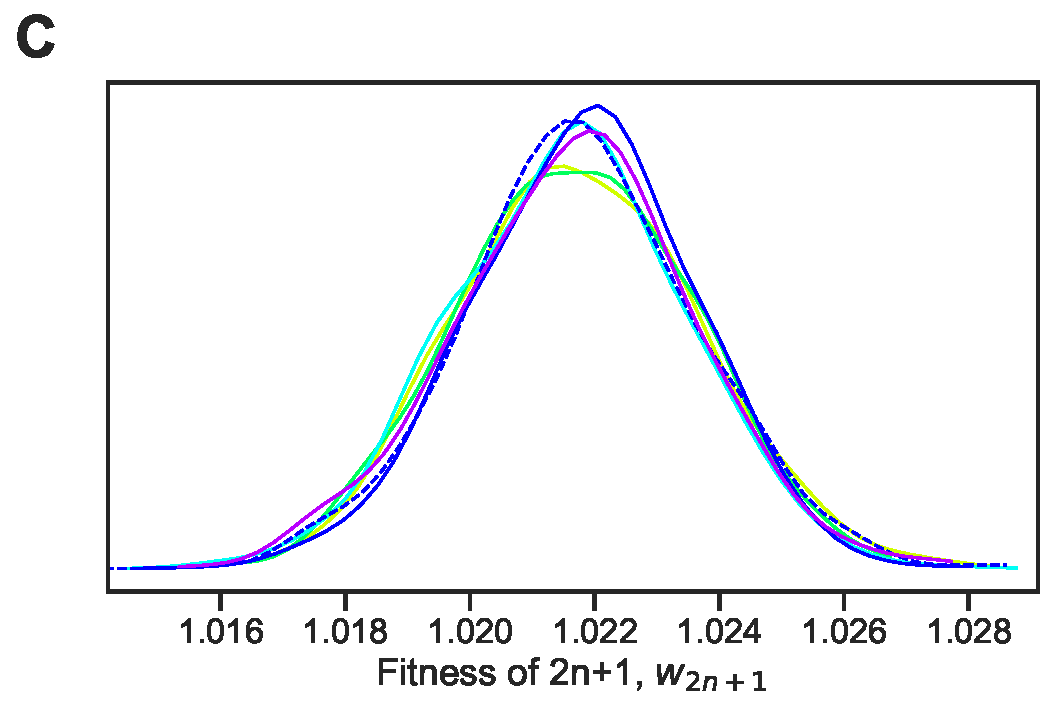
\includegraphics[width=0.325\textwidth]{../figures/runs-C.pdf}      
      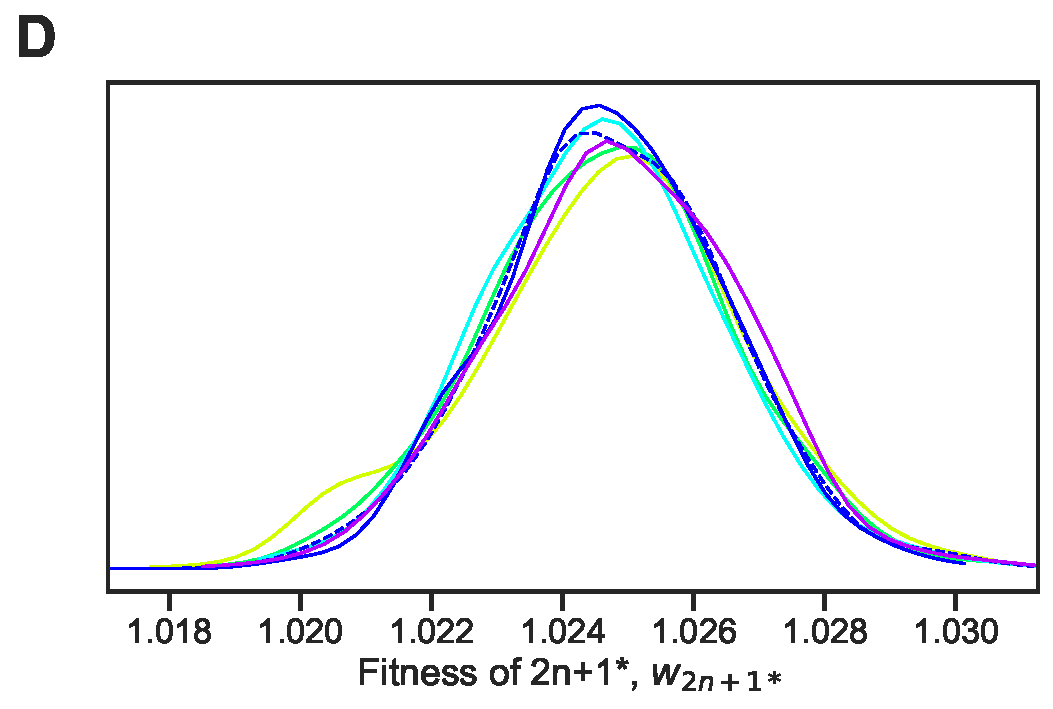
\includegraphics[width=0.325\textwidth]{../figures/runs-D.pdf}      
      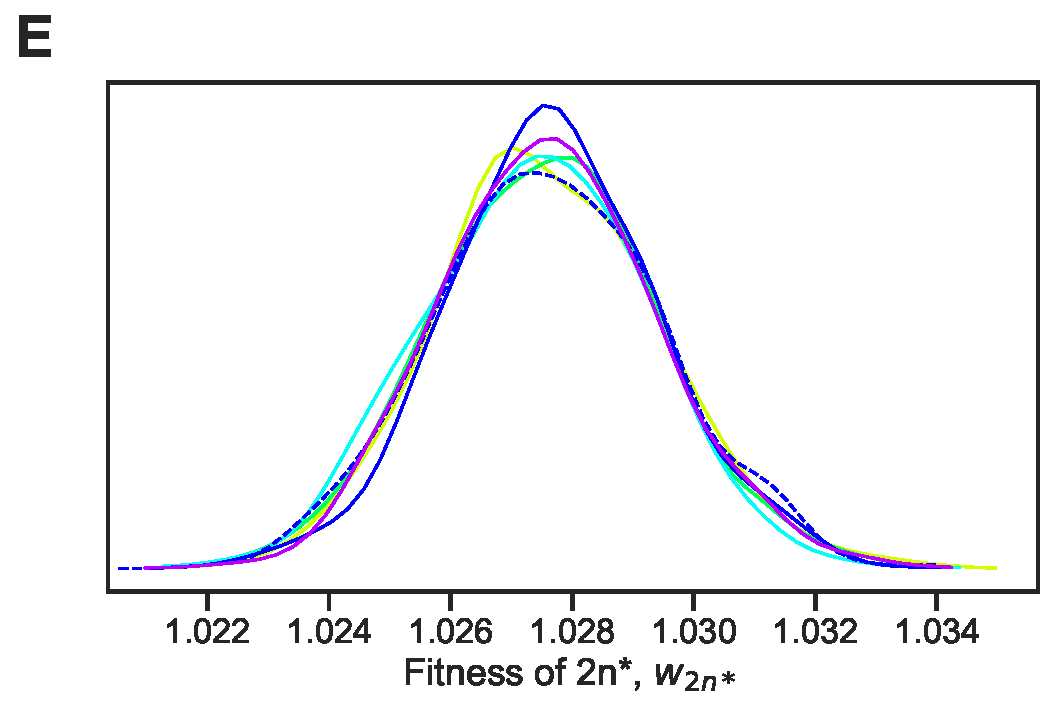
\includegraphics[width=0.325\textwidth]{../figures/runs-E.pdf} 
       \caption{
    \textbf{Posterior distribution validation.}
    The posterior distribution of model parameters is roughly the same regardless of the number of simulations (4-10,000 replicates) used to approximate the likelihood (\cref{eq:heatstress-likelihood}).
    } 
     
     \label{fig:seeds}
 \end{figure}
 
 % Fig tau comparisons
%% generated with diff-tau.ipynb
% TODO IK 10_000 reps is mocked, should be rerunned and fixed
\begin{figure}[h!]
  \centering
  \begin{subfigure}{0.45\textwidth}
      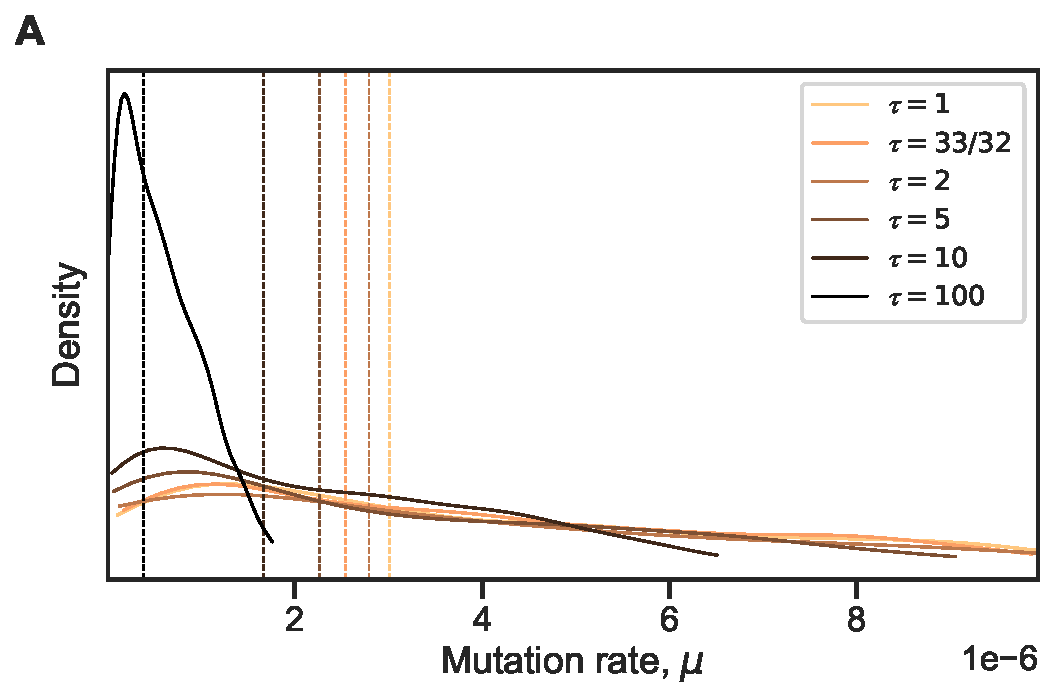
\includegraphics[width=\textwidth]{../figures/tau-A.pdf}      
  \end{subfigure}
  \begin{subfigure}{0.45\textwidth}
      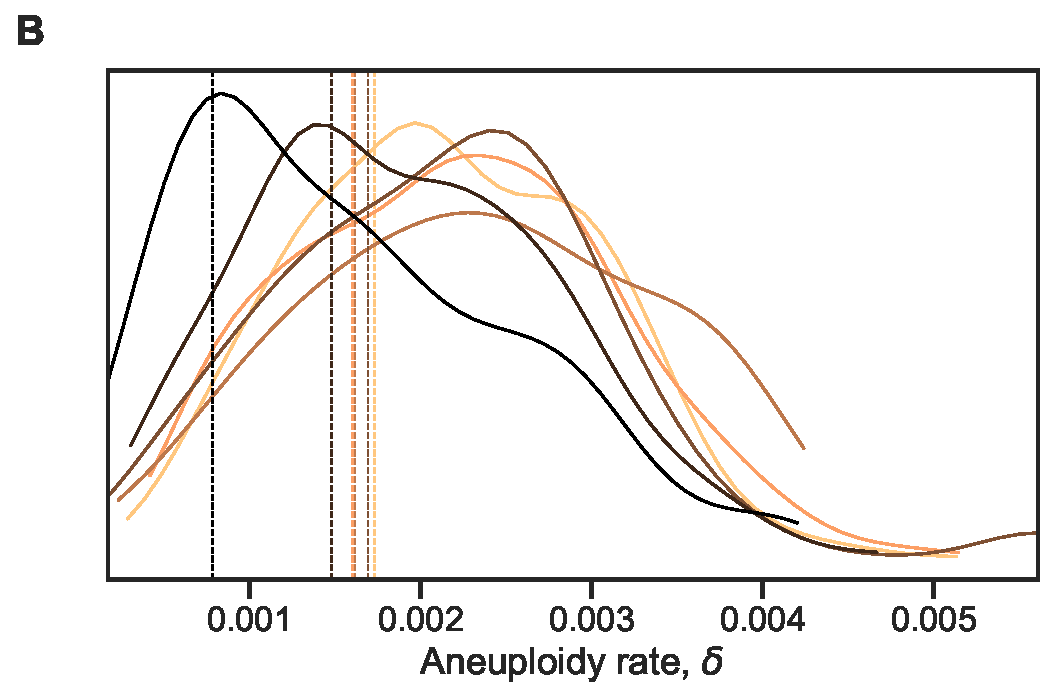
\includegraphics[width=\textwidth]{../figures/tau-B.pdf}      
  \end{subfigure}
  \\
   \begin{subfigure}{0.325\textwidth}
      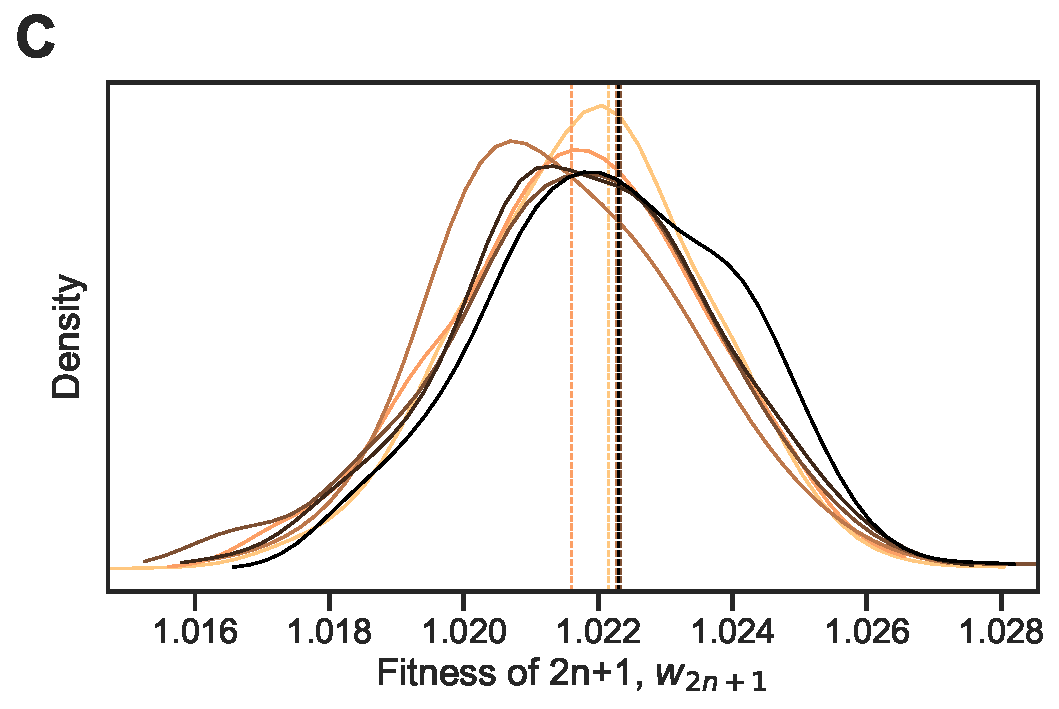
\includegraphics[width=\textwidth]{../figures/tau-C.pdf}      
  \end{subfigure}
    \begin{subfigure}{0.325\textwidth}
      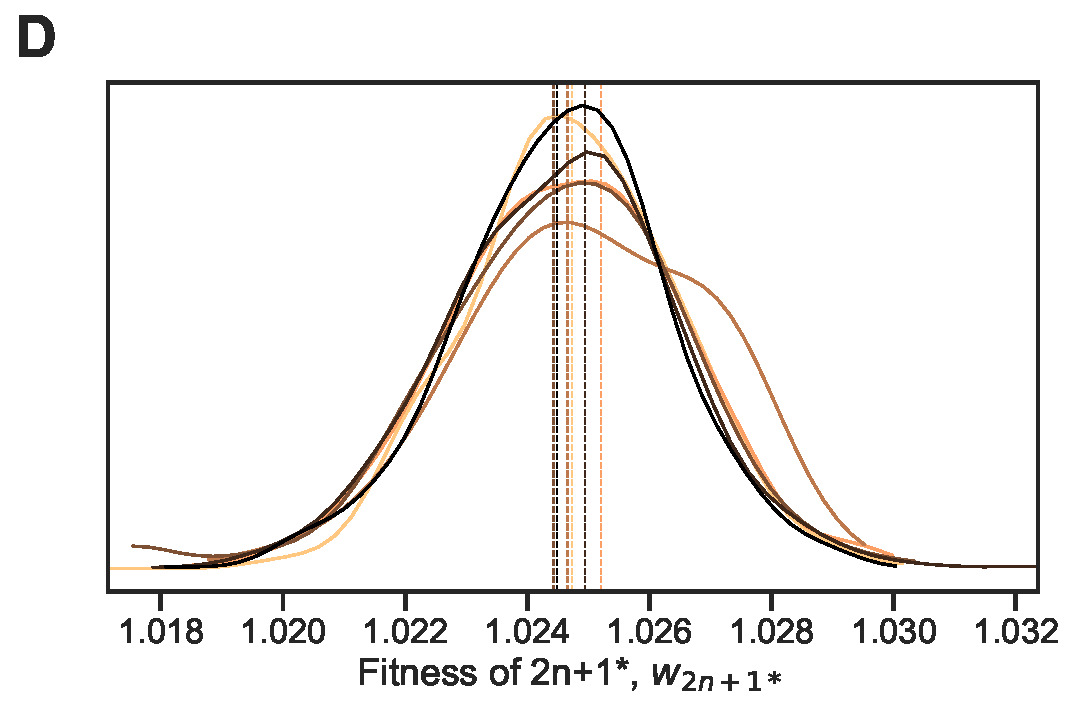
\includegraphics[width=\textwidth]{../figures/tau-D.pdf}      
  \end{subfigure}
    \begin{subfigure}{0.325\textwidth}
      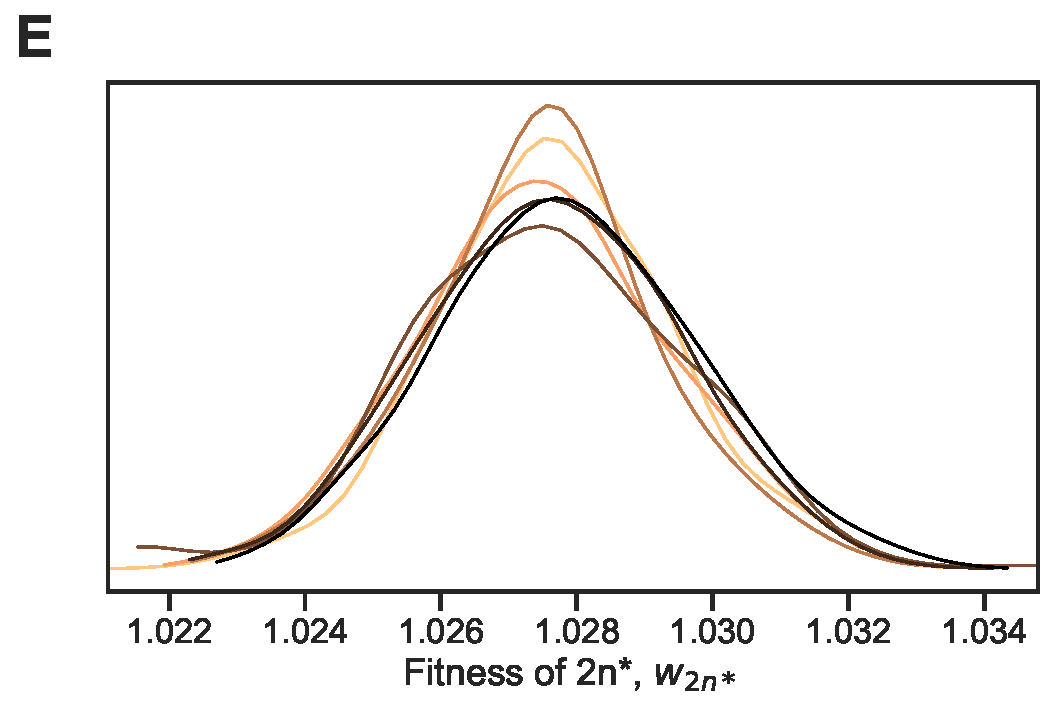
\includegraphics[width=\textwidth]{../figures/tau-E.pdf}      
  \end{subfigure}
  \\
  \begin{subfigure}{0.325\textwidth}
      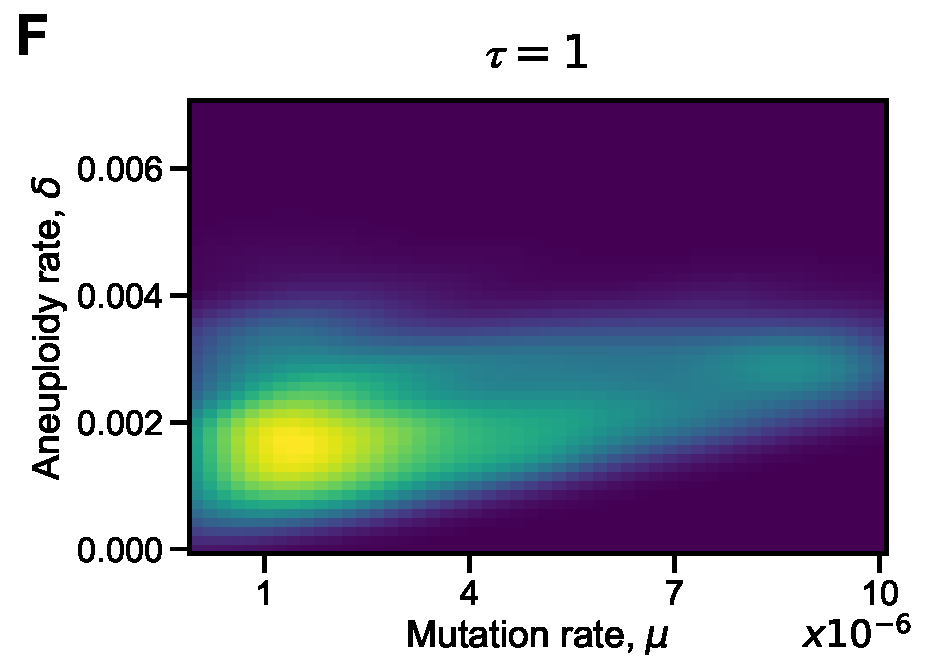
\includegraphics[width=\textwidth]{../figures/tau-joint-F.pdf}      
  \end{subfigure}
\begin{subfigure}{0.325\textwidth}
      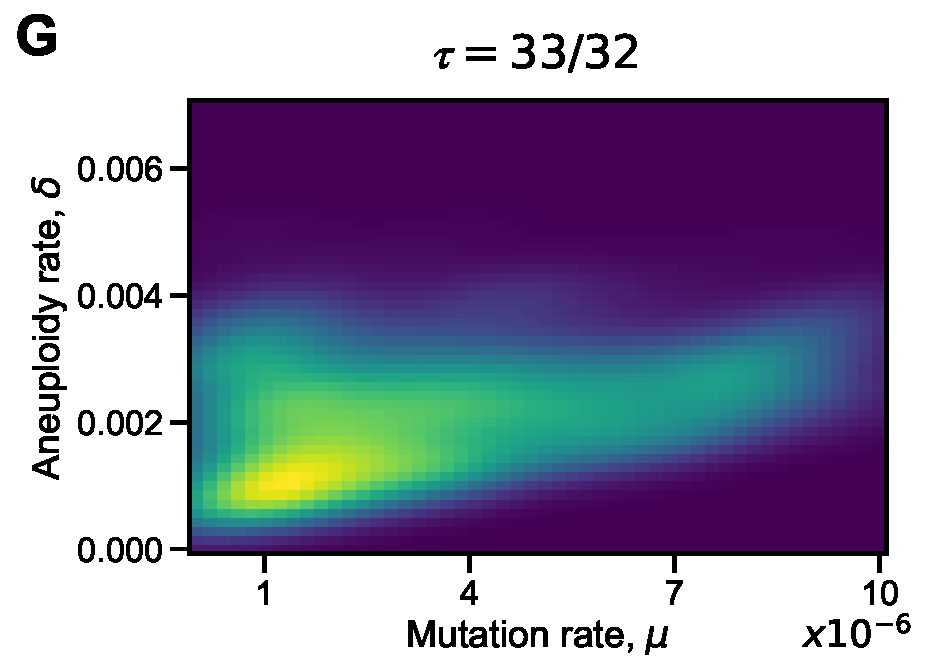
\includegraphics[width=\textwidth]{../figures/tau-joint-G.pdf}      
  \end{subfigure}
\begin{subfigure}{0.325\textwidth}
      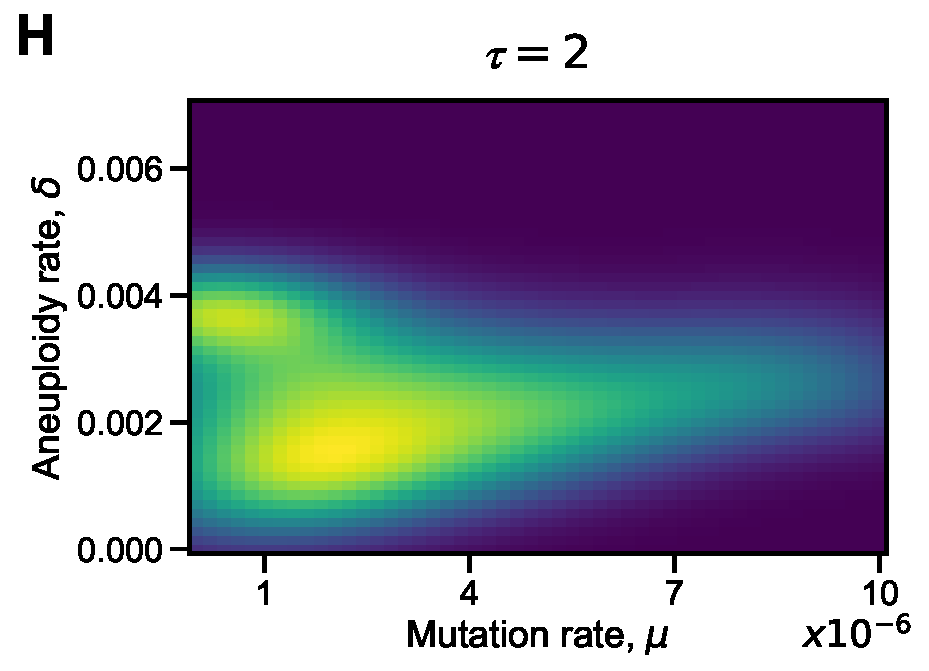
\includegraphics[width=\textwidth]{../figures/tau-joint-H.pdf}      
  \end{subfigure}
\begin{subfigure}{0.325\textwidth}
      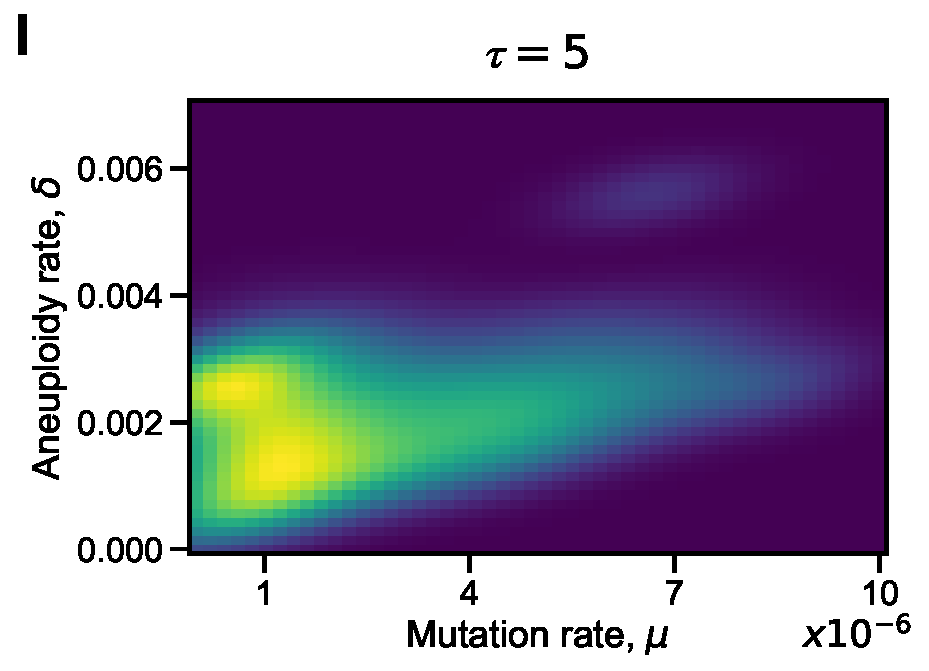
\includegraphics[width=\textwidth]{../figures/tau-joint-I.pdf}      
  \end{subfigure}
\begin{subfigure}{0.325\textwidth}
      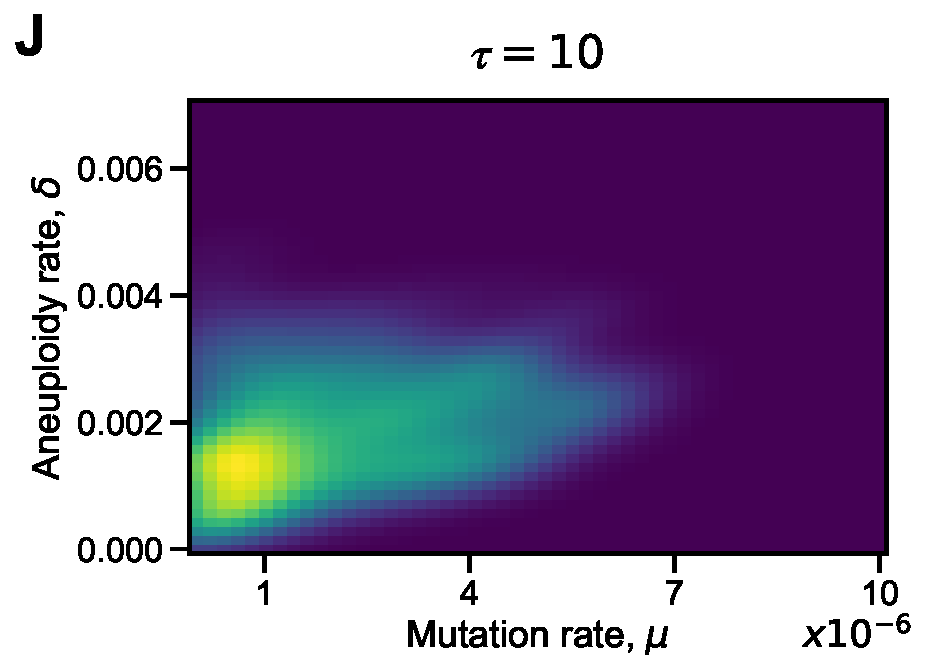
\includegraphics[width=\textwidth]{../figures/tau-joint-J.pdf}      
  \end{subfigure}
\begin{subfigure}{0.325\textwidth}
      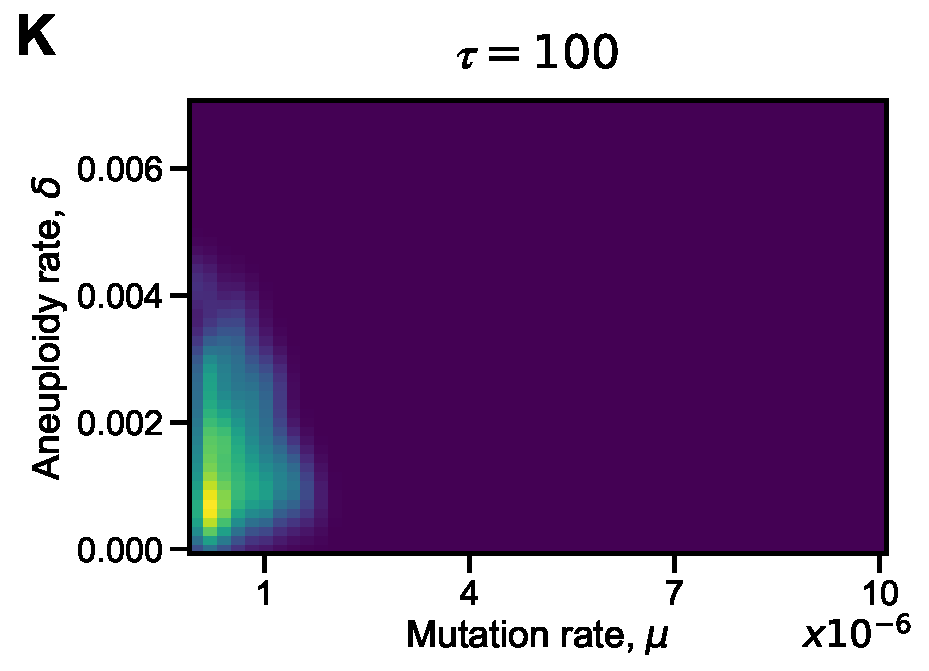
\includegraphics[width=\textwidth]{../figures/tau-joint-K.pdf}      
  \end{subfigure}
  \caption{
    \textbf{Model with elevated mutation rate in aneuploid cells.}  \textbf{(A-E)} The inferred posterior distributions for models with different values of $\tau$, the fold-increase in mutation rate in aneuploid cells (\anwt\ and \anmt). Vertical dashed lines represent MAP (maximum a posteriori) of each distribution. When the increase in mutation rate is high, $\tau=10$ and $\tau=100$, the inferred mutation (A) and aneuploidy (B) rate tends to be lower. 
    \textbf{(F-K)} The inferred joint posterior distribution of mutation rate ($\mu$) and aneuploidy rate ($\delta$) with different $\tau$ values (dark purple and bright yellow for low and high density, respectively).
  \label{fig:tau}
  }
  \end{figure}
  
  
% Fig mu comparisons
%% generated with diff-mutation-rate.ipynb
\begin{figure}[h!]
  \centering
  \begin{subfigure}{0.45\textwidth}
      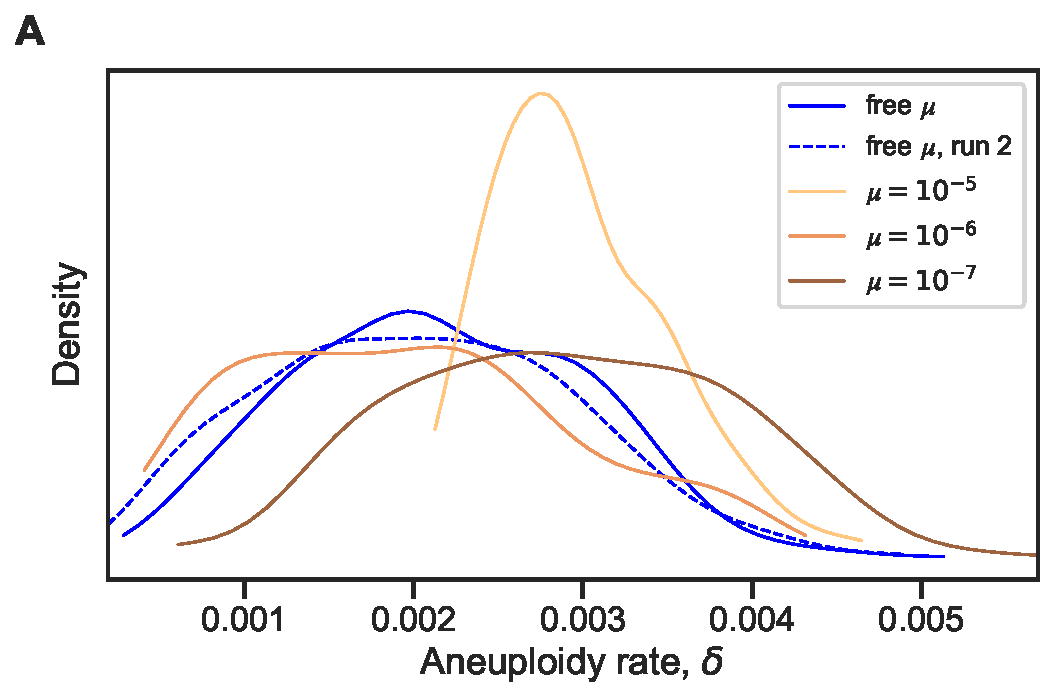
\includegraphics[width=\textwidth]{../figures/mu-A.pdf}      
  \end{subfigure}
  \begin{subfigure}{0.45\textwidth}
      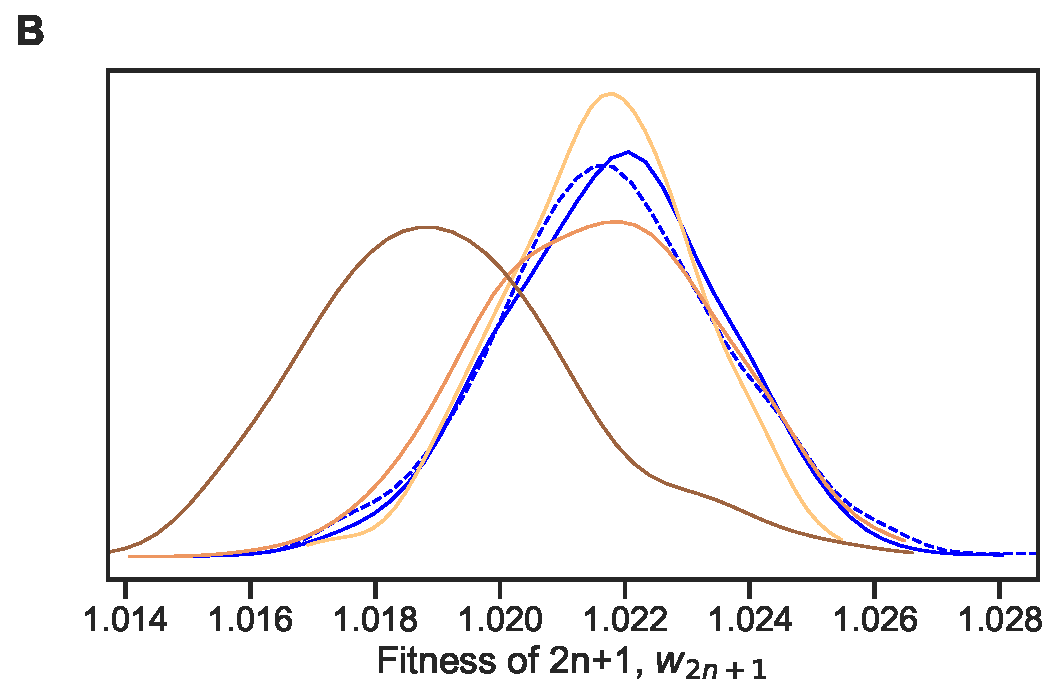
\includegraphics[width=\textwidth]{../figures/mu-B.pdf}      
  \end{subfigure}
  \\
   \begin{subfigure}{0.45\textwidth}
      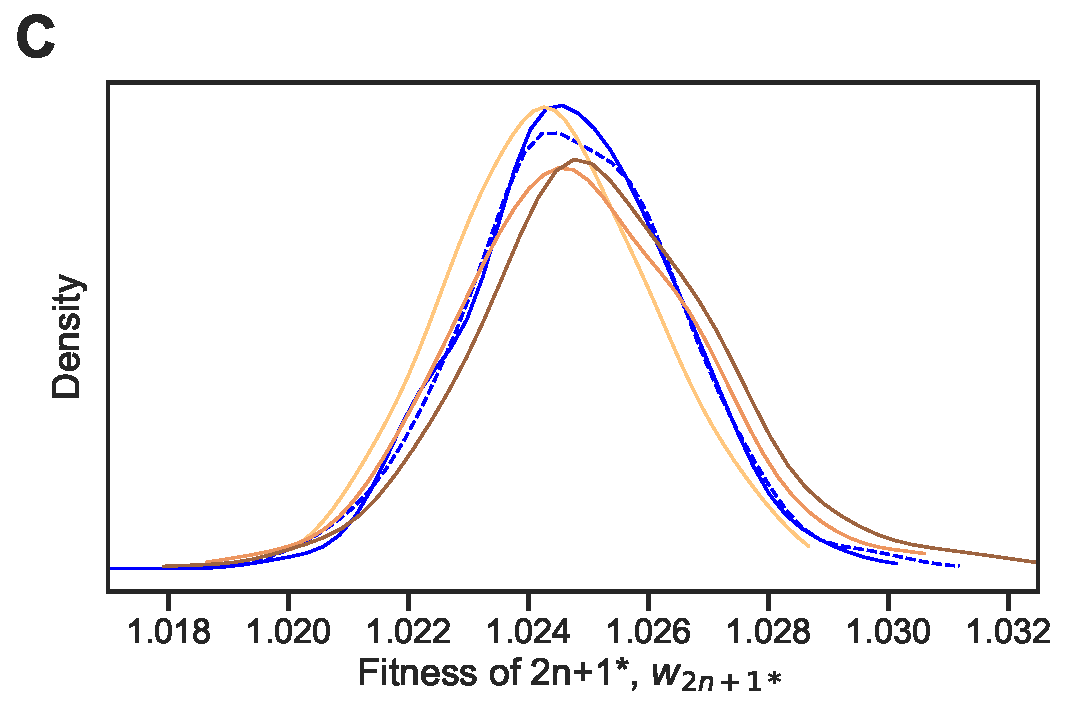
\includegraphics[width=\textwidth]{../figures/mu-C.pdf}      
  \end{subfigure}
    \begin{subfigure}{0.45\textwidth}
      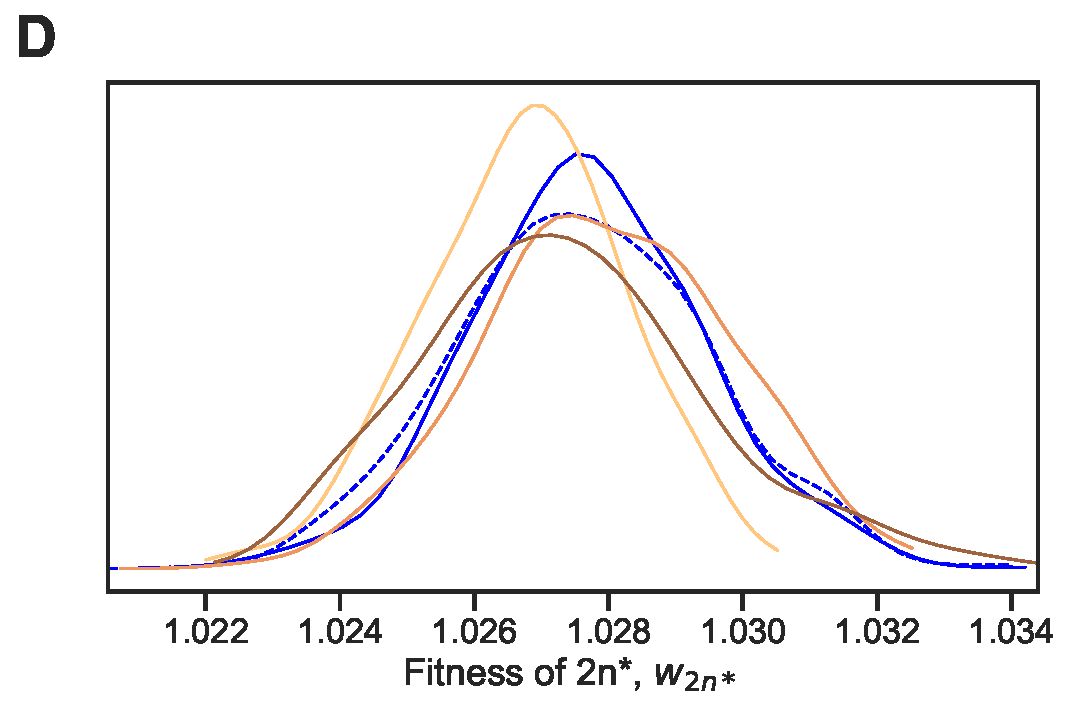
\includegraphics[width=\textwidth]{../figures/mu-D.pdf}      
    \end{subfigure}
  \caption{
    \textbf{Model with fixed mutation rate.}  \textbf{(A-D)} The inferred posterior distributions for models with free and fixed mutation rate, $\mu$. The MAP (maximum a posteriori) and 50\% HDI (highest density interval) for each model are: 
\textbf{free $\boldsymbol{\mu}$, run 1:}
$\delta=2.749\cdot10^{-3}\ [1.476\cdot10^{-3}-2.822\cdot10^{-3}]$,
$w_{\anwt}=1.022\ [1.021-1.023]$,
$w_{\anmt}=1.025\ [1.023-1.026]$,
$w_{\eumt}=1.027\ [1.026-1.029]$;
\textbf{free $\boldsymbol{\mu}$, run 2:}
$\delta=1.938\cdot10^{-3}\ [1.338\cdot10^{-3}-2.748\cdot10^{-3}]$,
$w_{\anwt}=1.022\ [1.02-1.023]$,
$w_{\anmt}=1.025\ [1.023-1.026]$,
$w_{\eumt}=1.027\ [1.026-1.029]$;
\textbf{$\boldsymbol{\mu=10^{-5}}$:}
$\delta=3.089\cdot10^{-3}\ [2.412\cdot10^{-3}-3.169\cdot10^{-3}]$,
$w_{\anwt}=1.022\ [1.021-1.023]$,
$w_{\anmt}=1.024\ [1.023-1.026]$,
$w_{\eumt}=1.027\ [1.026-1.028]$;
\textbf{$\boldsymbol{\mu=10^{-6}}$:}
$\delta=1.413\cdot10^{-3}\ [1.04\cdot10^{-3}-2.529\cdot10^{-3}]$,
$w_{\anwt}=1.021\ [1.02-1.023]$,
$w_{\anmt}=1.024\ [1.023-1.026]$,
$w_{\eumt}=1.028\ [1.026-1.029]$;
\textbf{$\boldsymbol{\mu=10^{-7}}$:}
$\delta=3.4\cdot10^{-3}\ [2.043\cdot10^{-3}-3.578\cdot10^{-3}]$,
$w_{\anwt}=1.019\ [1.017-1.02]$,
$w_{\anmt}=1.026\ [1.024-1.027]$,
$w_{\eumt}=1.027\ [1.026-1.029]$.
\label{fig:mu}
  }
  \end{figure}

 
%TODO YR read this 
%% generated with WAIC.ipynb 
\begin{table}[h]
\centering
\caption{
\textbf{WAIC values for various model specifications.}}
\pgfplotstabletypeset[
    col sep=semicolon,
    string type,
    every head row/.style={before row=\hline,after row=\hline},
    every last row/.style={after row=\hline},
    ]{../figures/Table_WAIC.csv} 
\caption*{
	WAIC (widely applicable information criterion, \cref{eq:WAIC})~\citep{gelman2013bayesian} values for models with different configurations. WAIC values are scaled as a deviance measure: lower values imply higher predictive accuracy and a difference of 2 is a popular threshold for model comparison~\citep{Kass1995}.
} 
\label{table:WAIC}
\end{table}

\end{document}  